\documentclass[a4paper,10pt]{article}
\usepackage[utf8]{inputenc}
\usepackage[a4paper,
            bindingoffset=0.2in,
            left=1in,
            right=1in,
            top=1in,
            bottom=1in,
            footskip=.25in]{geometry}

%###############################################################################

%\input{~/layout/global_layout}


%###############################################################################

% packages begin

\usepackage[
  backend=biber,
  sortcites=true,
  style=alphabetic,
  eprint=true,
  backref=true
]{biblatex}
\addbibresource{bibliographie.bib}
\usepackage[acronym]{glossaries}

\usepackage{euscript}[mathcal]
% e.g. \mathcal{A} for fancy letters in mathmode
\usepackage{amsmath,amssymb,amstext,amsthm}

\usepackage{mdframed}
\newmdtheoremenv[nobreak=true]{problem}{Problem}[subsection]
\newmdtheoremenv[nobreak=true]{claim}{Claim}[subsection]
\newtheorem{definition}{Definition}[subsection]
\newtheorem{lemma}{Lemma}[claim]
\newtheorem{plemma}{Lemma}[problem]

\usepackage{mathtools}
\DeclarePairedDelimiter\ceil{\lceil}{\rceil}
\DeclarePairedDelimiter\floor{\lfloor}{\rfloor}

\usepackage{enumerate}
\usepackage[pdftex]{graphicx}
\usepackage{subcaption}
% 'draft' für schnelleres rendern mitübergeben -> [pdftex, draft]
% dadruch wird nicht das bild mitgerendered, sondern nur ein kasten mit bildname -> schont ressourcen

\usepackage{hyperref}

\usepackage{tikz}
\usetikzlibrary{arrows,automata,matrix,positioning,shapes}

% for adding non-formatted text to include source-code
\usepackage{listings}
\lstset{language=Python,basicstyle=\footnotesize}
% z.B.:
% \lstinputlisting{source_filename.py}
% \lstinputlisting[lanugage=Python, firstline=37, lastline=45]{source_filename.py}
%
% oder
%
% \begin{lstlisting}[frame=single]
% CODE HERE
%\end{lstlisting}
\usepackage{algorithm}
\usepackage{algpseudocode}

\usepackage{wasysym}

\usepackage{titling}
\usepackage{titlesec}
\usepackage[nocheck]{fancyhdr}
\usepackage{lastpage}

\usepackage{kantlipsum}
\usepackage[colorinlistoftodos,prependcaption,textsize=tiny]{todonotes}

% packages end
%###############################################################################

\pretitle{% add some rules
  \begin{center}
    \LARGE\bfseries
} %, make the fonts bigger, make the title (only) bold
\posttitle{%
  \end{center}%
  %\vskip .75em plus .25em minus .25em% increase the vertical spacing a bit, make this particular glue stretchier
}
\predate{%
  \begin{center}
    \normalsize
}
\postdate{%
  \end{center}%
}

\titleformat*{\section}{\Large\bfseries}
\titleformat*{\subsection}{\large\bfseries}
\titleformat*{\subsubsection}{\normalsize\bfseries}

\titleformat*{\paragraph}{\Large\bfseries}
\titleformat*{\subparagraph}{\large\bfseries}

%###############################################################################

\pagestyle{fancy}
\fancyhf{}
% l=left, c=center, r=right; e=even_pagenumber, o=odd_pagenumber; h=header, f=footer
% example: [lh] -> left header, [lof,ref] -> fotter left when odd, right when even
%\fancyhf[lh]{}
%\fancyhf[ch]{}
%\fancyhf[rh]{}
%\fancyhf[lf]{}
\fancyhf[cf]{\footnotesize Page \thepage\ of \pageref*{LastPage}}
%\fancyhf[rf]{}
\renewcommand{\headrule}{} % removes horizontal header line

% Fotter options for first page

\fancypagestyle{firstpagestyle}{
  \renewcommand{\thedate}{\textmd{}} % removes horizontal header line
  \fancyhf{}
  \fancyhf[lh]{\ttfamily M.Sc. Computer Science\\KTH Royal Institute of Technology}
  \fancyhf[rh]{\ttfamily Period 4\\\today}
  \fancyfoot[C]{\footnotesize Page \thepage\ of \pageref*{LastPage}}
  \renewcommand{\headrule}{} % removes horizontal header line
}
%###############################################################################

\newcommand\extrafootertext[1]{%
    \bgroup
    \renewcommand\thefootnote{\fnsymbol{footnote}}%
    \renewcommand\thempfootnote{\fnsymbol{mpfootnote}}%
    \footnotetext[0]{#1}%
    \egroup
}

%###############################################################################

\title{
  \normalsize{DD2356 VT25 Methods in}\\
  \normalsize{High Performance Computing}\\
  \large{Assignment 4}
}
\author{
  \small Rishi Vijayvargiya\textsuperscript{\textdagger}\\[-0.75ex]
%  \footnotesize\texttt{MN: }\\[-1ex]
  \scriptsize\texttt{rishiv@kth.se}
  \and
  \small Paul Mayer\textsuperscript{\textdagger}\\[-0.75ex]
%  \footnotesize\texttt{MN: }\\[-1ex]
  \scriptsize\texttt{pmayer@kth.se}
  \and
  \small Lennard Herud \textsuperscript{\textdagger}\\[-0.75ex]
%  \footnotesize\texttt{MN: }\\[-1ex]
  \scriptsize\texttt{herud@kth.se}
}
\date{}

%###############################################################################
% define Commands

\newcommand{\N}{\mathbb{N}}
\newcommand{\R}{\mathbb{R}}
\newcommand{\Z}{\mathbb{Z}}
\newcommand{\I}{\mathbb{I}}

\newcommand{\E}{\mathbb{E}}
\newcommand{\Prob}{\mathbb{P}}

\renewcommand{\epsilon}{\varepsilon}

%###############################################################################
\makeatletter
\renewcommand*{\@fnsymbol}[1]{\ensuremath{\ifcase#1\or \dagger\or \ddagger\or
   \mathsection\or \mathparagraph\or \|\or **\or \dagger\dagger
   \or \ddagger\ddagger \else\@ctrerr\fi}}
\makeatother
%###############################################################################

\begin{document}
\maketitle
\extrafootertext{\textsuperscript{\textdagger}Authors made equal contribution to the project}
\thispagestyle{firstpagestyle}
\vspace{1em}

% content begin
%

\section*{Prefix}
The code for our project can be found at this location: \url{https://github.com/paulmyr/DD2356-MethodsHPC/tree/master/4_mpi}. 

\tableofcontents
\newpage

\section{1D Halo Exchange in a Wave Equation Simulation}
\subsection{MPI Implementation}
The MPI implementation can be found in the file \verb|halo_parallel.c| \href{https://github.com/paulmyr/DD2356-MethodsHPC/blob/master/4_mpi/ex1/halo_parallel.c}{here}. Our parallelization strategy using MPI involves three main components. 

Firstl, we have the root process (with rank 0) initialize the entire \verb|u| and \verb|u_prev| variables, and then distribute them to the other processes (and to itself) using the \verb|MPI_Scatter| method. This can be seen in the \verb|initialize_and_distribute_data| function of the file \href{https://github.com/paulmyr/DD2356-MethodsHPC/blob/master/4_mpi/ex1/halo_parallel.c#L77}{here}. 

Second, in the main computation loop, we perform the halo exchange using the \verb|Sendrecv| method. To be able to perform halo exchanges in a simple manner, we first create a 1D cartesian topology assigns each chunk of the array to a process using the \verb|MPI_Cart_create| method, where the dimensions are provided by the output of the \verb|MPI_Dims_create| method. This topology is used to get reliable information about the left and right neighbours of each process (using the \verb|MPI_Cart_shift| method) to perform the halo exchange with processes responsible for the neighbouring chunks. In each step of the loop, we perform the halo exchanges, followed by the main computation in \verb|compute_step| (found \href{https://github.com/paulmyr/DD2356-MethodsHPC/blob/master/4_mpi/ex1/halo_parallel.c#L14}{here}). 

The \verb|compute_step| method has special cases for processes handling the first and last chunk. This is because the first element and the last element of \verb|u| in the serial implementation do not seem to be impacted by the effects of the computations (the loop populating \verb|u_next| only updates from index 1 to \verb|N-1|). We made a discussion post about this. On observing behaviour, it seems that \verb|u_next[0]| and \verb|u_next[N-1]| were assigned to 0 in the serial implementation, so we explicitly do that here (both in the serial code and in the parallel version to ensure parity). 

Finally, to ensure validity of our results with the serial implementation, we print the current status of the grid at certain time-steps. To do this, we first introduce a \verb|MPI_Barrier| to ensure that all processes are at the same step in the computation. Then, we use \verb|MPI_Gather| to collect different chunks from the respective processes at the process with rank 0, which eventually prints the output to a file. \verb|MPI_Barrier| is also used at the end of the computation, to ensure that regardless of the print diagnostics (which are turned off when measuring runtime), the final state of the array \verb|u| is as expected. Then, the final output could be printed to a file if required. \textit{Note: When reporting runtime, we omit any I/O operations from occurring. However, the final} \verb|MPI_Barrier| \textit{ call is kept within the timing range for correctness, along with the code required to accumulate the final state of the array from all process to the root process with rank 0}. 

\subsection{Correctness of Parallel Implementation}
The output generated for $N = 6.4\text{ million}$ and $STEPS = 5000$ can be seen below for both the serial and parallel implementations. We plot at every 500th timestep, followed by a final plot after the computation loop. As can be seen visually from Figure \ref{fig:ex1_parallel_output} and \ref{fig:ex1_serial_output}, the outputs look identical. 

\begin{figure}[h]
     \centering
     \begin{subfigure}[b]{0.45\textwidth}
        \centering
        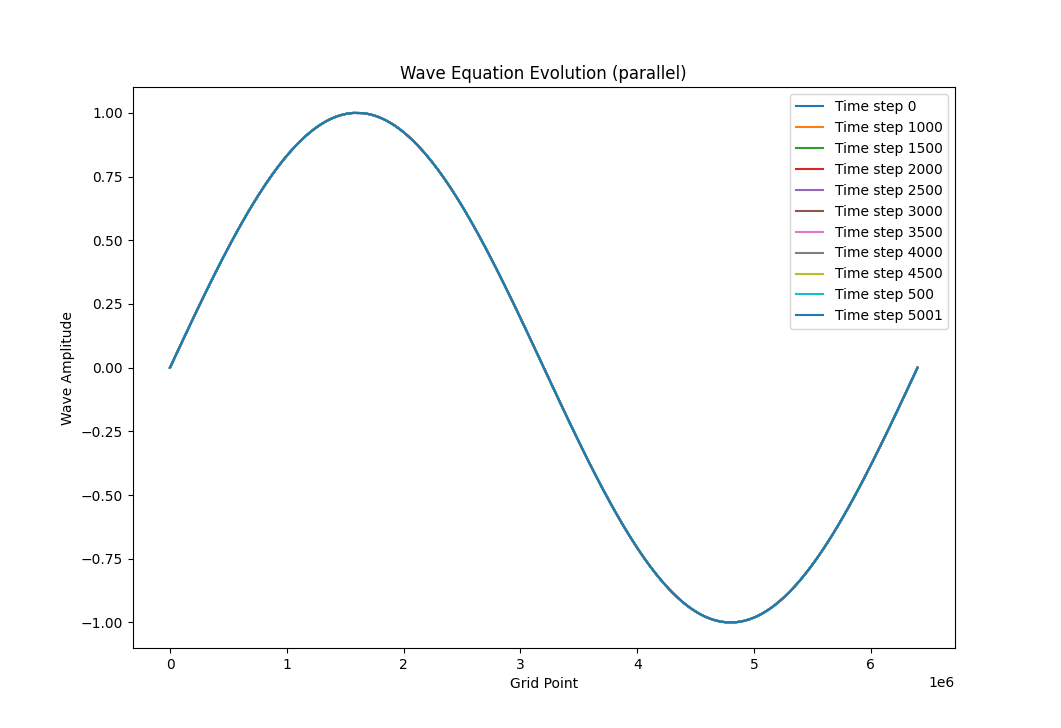
\includegraphics[width=\linewidth]{img/ex1/wave_vis_parallel.png}
        \caption{Parallel Output}
        \label{fig:ex1_parallel_output}
     \end{subfigure}
     \hfill
     \begin{subfigure}[b]{0.45\textwidth}
        \centering
        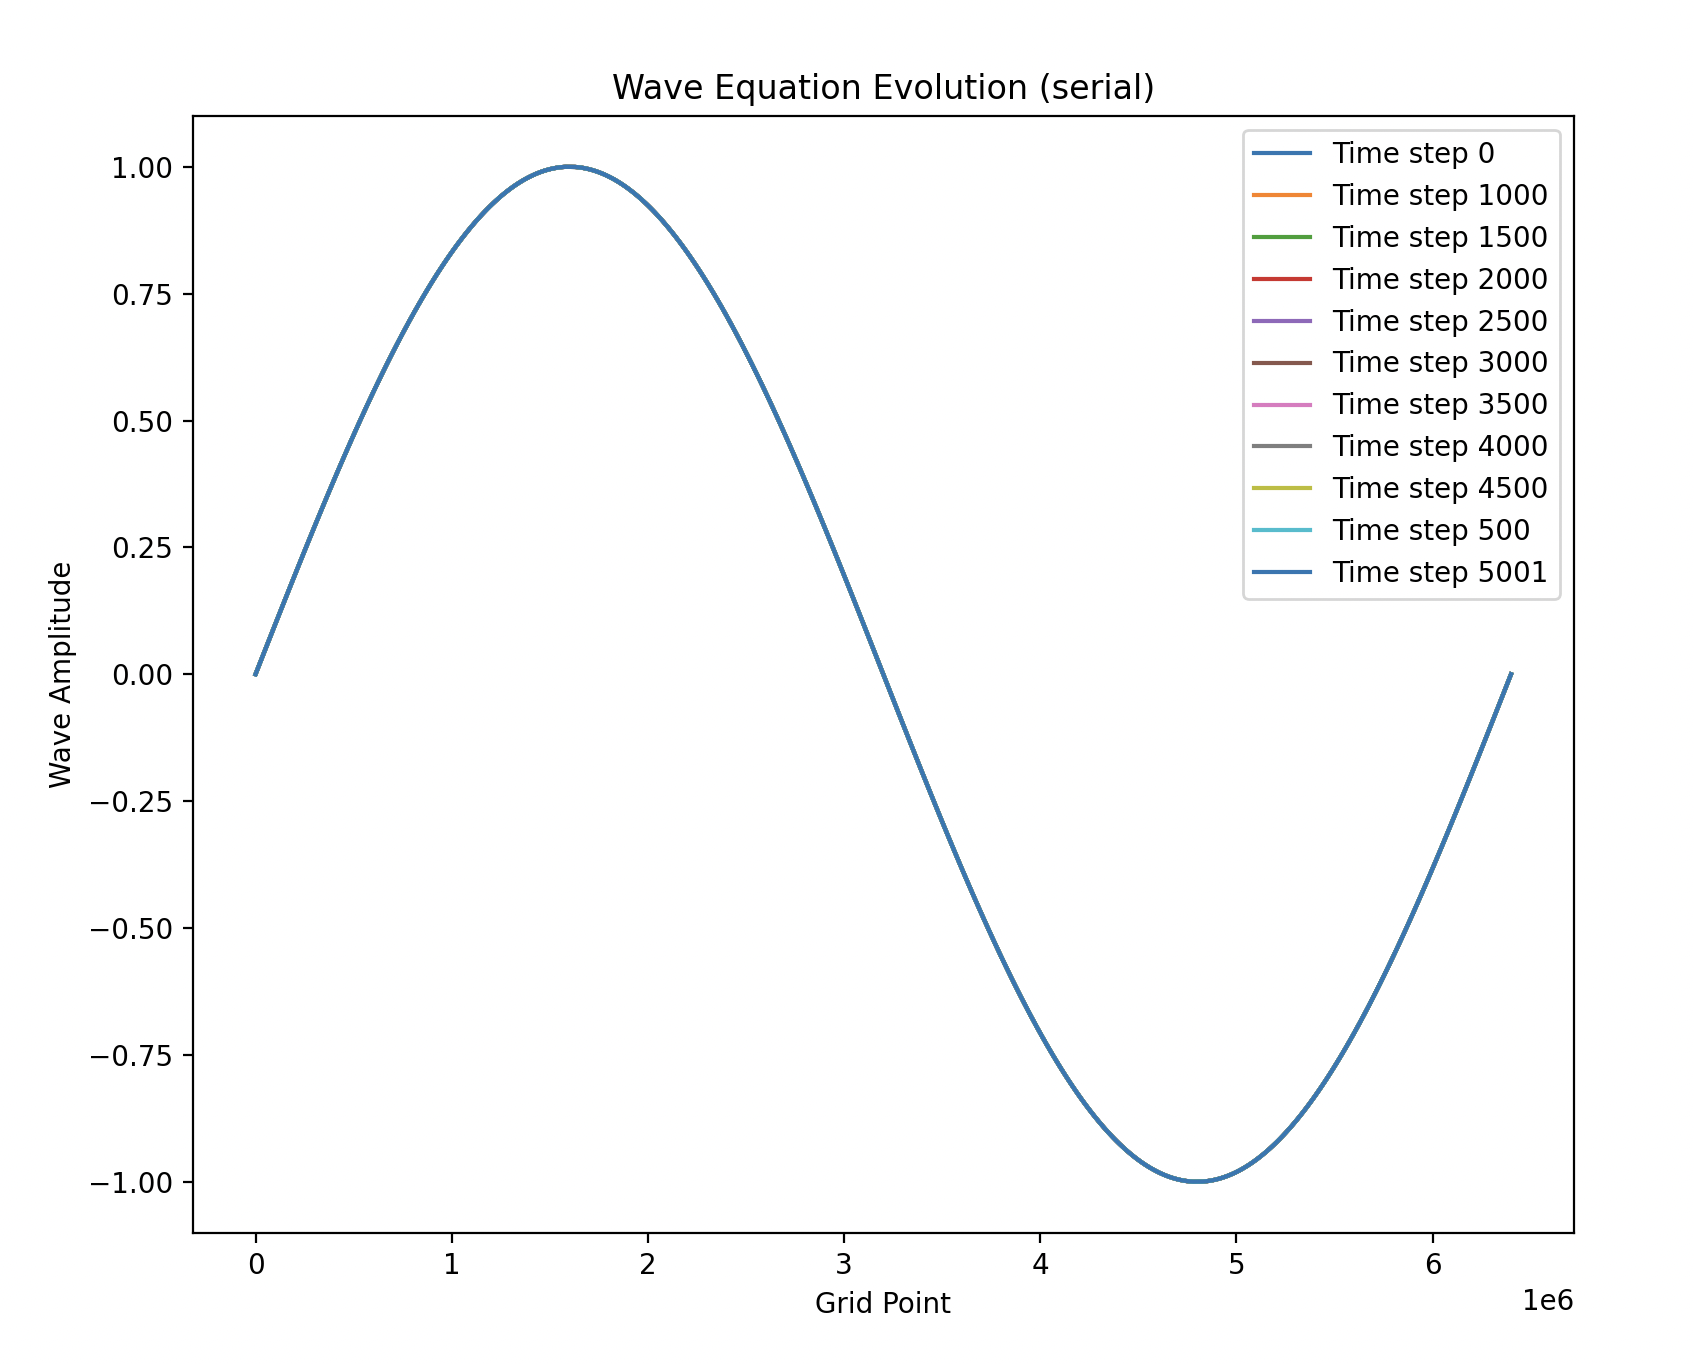
\includegraphics[width=\linewidth]{img/ex1/wave_vis_serial.png}
        \caption{Serial Output}
        \label{fig:ex1_serial_output}
     \end{subfigure}
  \caption{Parallel and Serial Outputs}
\end{figure}

To generate this plot, the following command can be run form under the \verb|ex1/| directory: 

\begin{center}
\verb|python3 visualize.py --mode {parallel/serial}|
\end{center}

To further ensure that the outputs were identical, a bash script was created: \verb|verify_outputs.sh|. This individually checks for diffs between the parallel and the serial implmenetation output, failing if the parallel and serial files for any timestamp are not identical. It can be found \href{https://github.com/paulmyr/DD2356-MethodsHPC/blob/master/4_mpi/ex1/verify_outputs.sh}{here} and is run using \verb|sh verify_outputs.sh| from under the \verb|ex1/| directory. 

\subsection{Runtime Analysis}
For this analysis, we used $N = 6.4\text{ million}$ and $STEPS = 5000$. The plots were generated with the python file \verb|plotting.py| in the \verb|ex1/| directory. The runtimes plotted below were obtained from the results in the \verb|ex1/outputs/runtimes| directory. 

\subsubsection{Runtime for Different Process Counts}
\label{sec:diff_process_counts}
The runtime for different number of processes compared to the serial implementation can be seen in Figure \ref{fig:ex1_process_counts}. For this, we used the configuration in the \verb|run_sim_vary_process.sh| file (found \href{https://github.com/paulmyr/DD2356-MethodsHPC/blob/master/4_mpi/ex1/run_sim_vary_process.sh}{here}), where we allocated 1 node with 64 tasks per node and 1 cpu per task.

\begin{figure}[H]
  \centering
  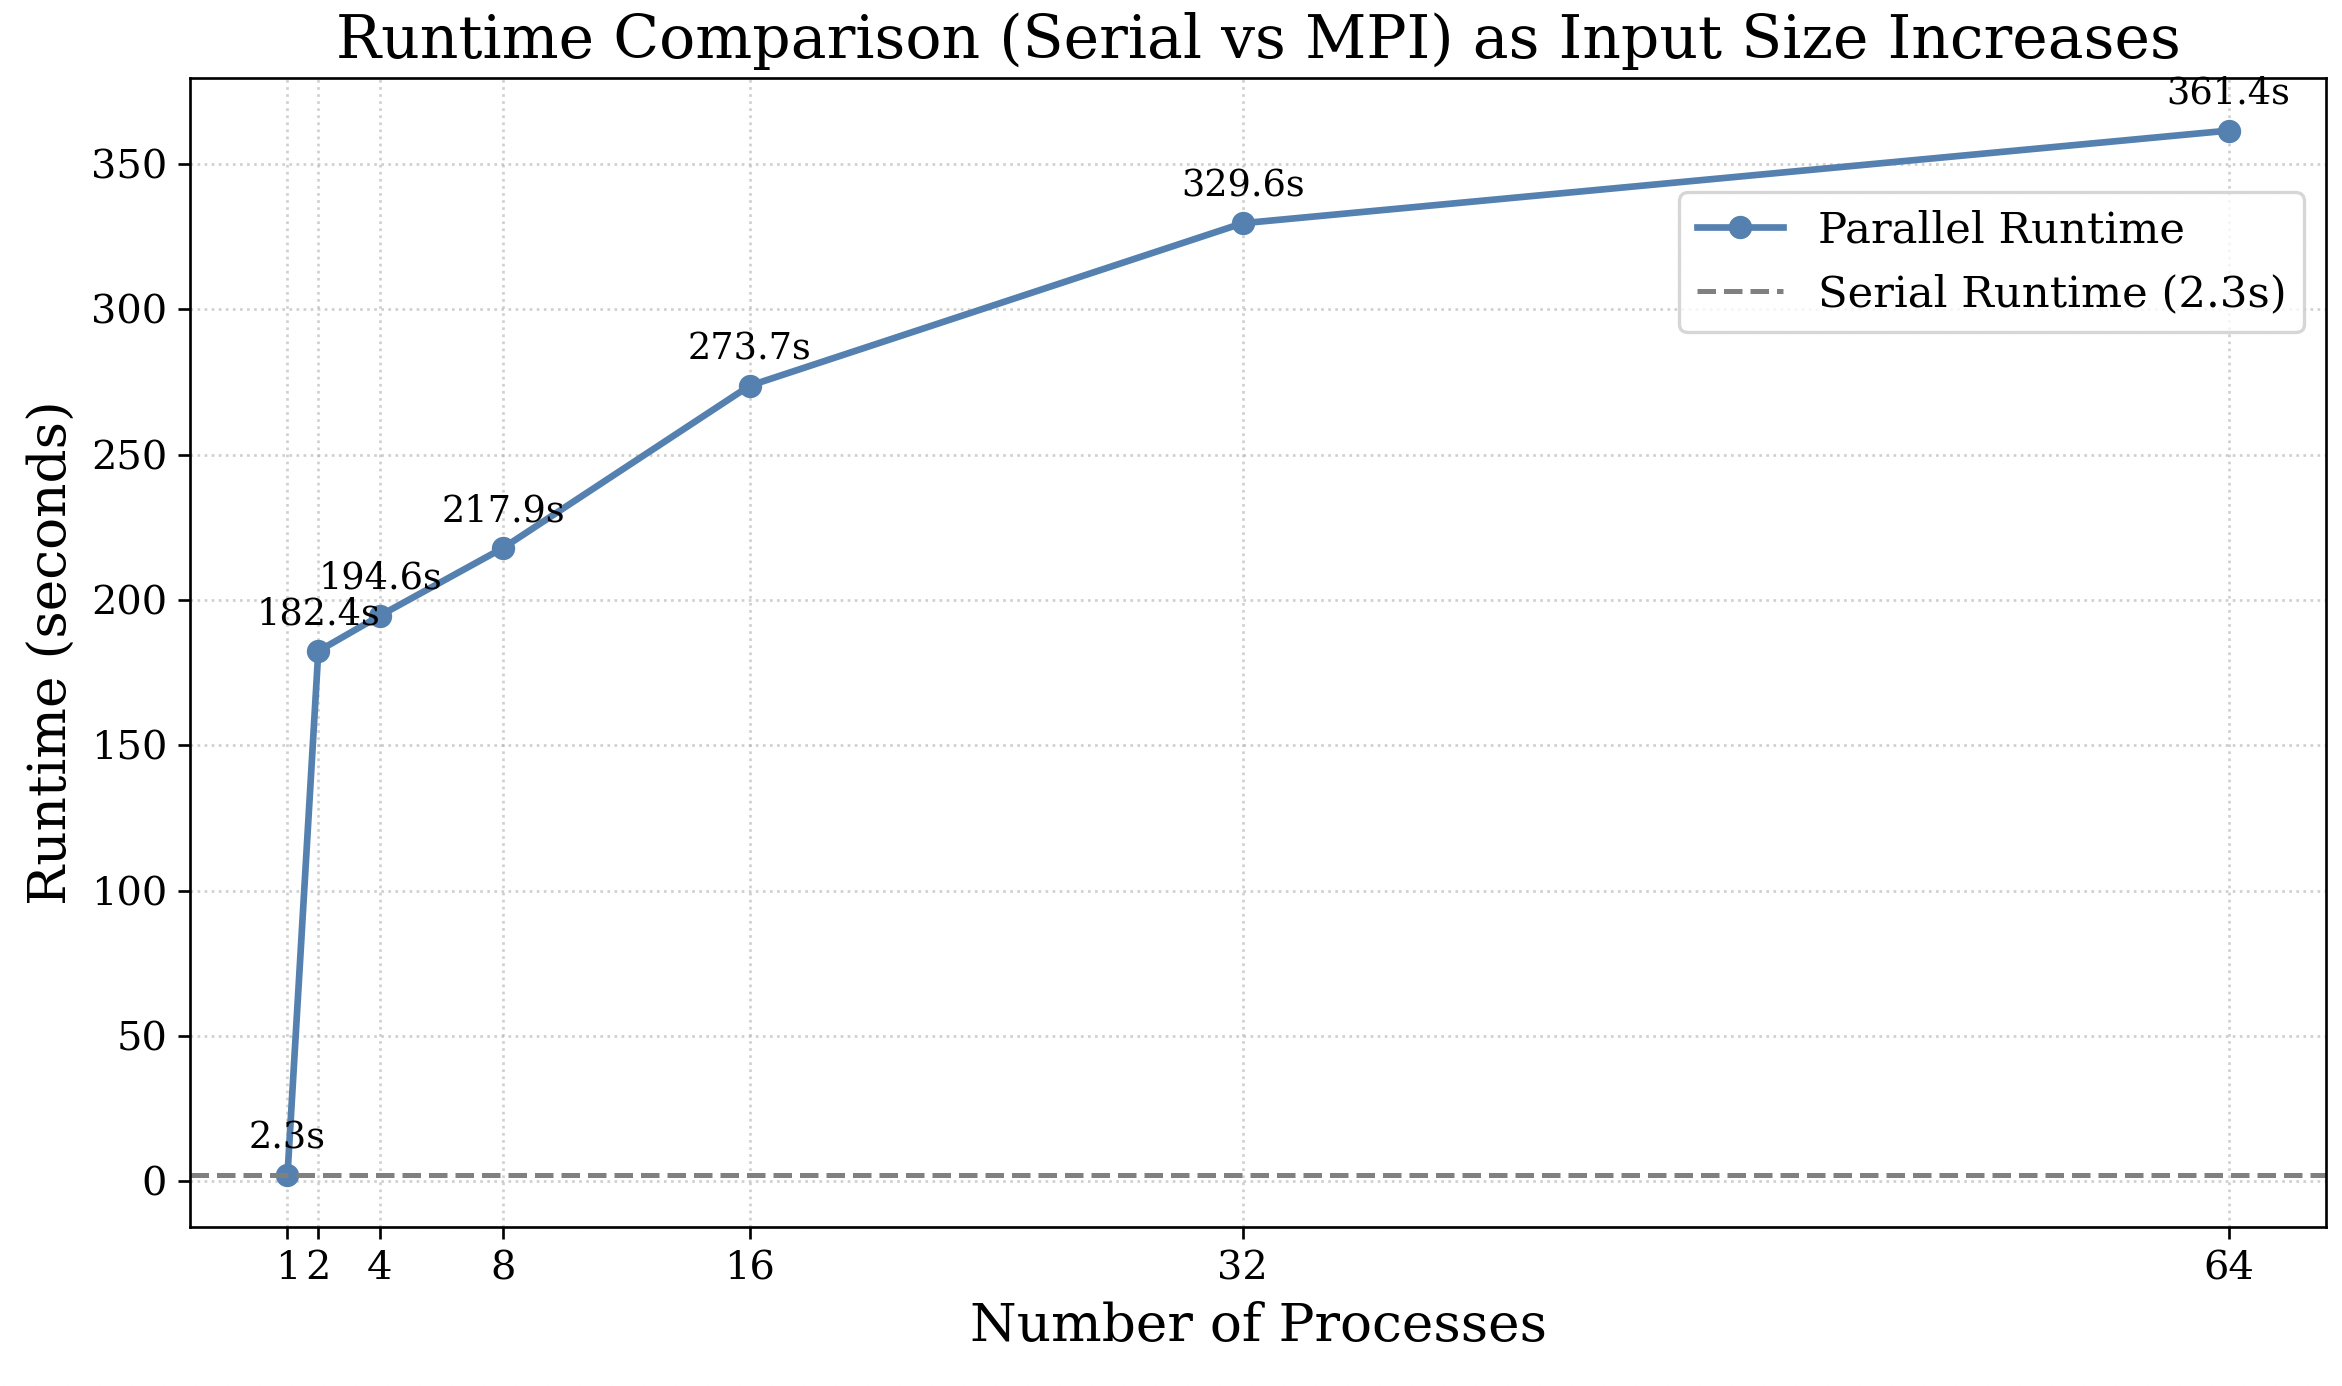
\includegraphics[width=0.9\textwidth]{img/ex1/serial_vs_mpi}
  \caption{Serial vs MPI Comparison for Different Process Counts}
  \label{fig:ex1_process_counts}
\end{figure}
As can be seen from the figure, after a similar and worse runtime for 1 and 2 processes respectively, the runtime for higher number of processes is lower compared to the serial runtime. We believe that the runtime for 1 or 2 processes could be attributed to the fact that there is greater MPI related overhead compared to the benefits achieved from the limited parallelism offered by 1 or 2 processes.
 
However, as the number of processes increase and the amount of work that needs to be done remains the same, we start to see the benefit of this work being done in parallel by multiple processes. The lowest runtime achieved seems to be from 4 processes, indicating that after this, the benfit of parallelism diminishes likely because of the greater MPI overhead (exchanging ghost cells between more processes, barrier at the end of computation waiting for more processes, etc). However, even after the slight increase, the runtime at 64 processes is considerably less than the serial, which shows the clear benefit of parallelism through MPI. 

\subsubsection{Runtime for Different Node Counts}
When chaning the number of nodes, we kept all other elements ($N$, $STEPS$, processes, etc) constant. We measured with a total of 32 processes, distributed equally amongst 1, 2, 4, and 8 nodes. This means that when operating with 2 nodes, each node had 16 processes, when using 4 nodes, each node had 8 processes, and so on. For each node count (except for 1 node, where we already had the runtime from above), the respective job-file is titled \verb|run_sim_nodes_<count>.sh| in the code. 

Given this setup, the runtime across different nodes compared to the serial implementation can be seen in Figure \ref{fig:ex1_node_counts}.
\begin{figure}[H]
  \centering
  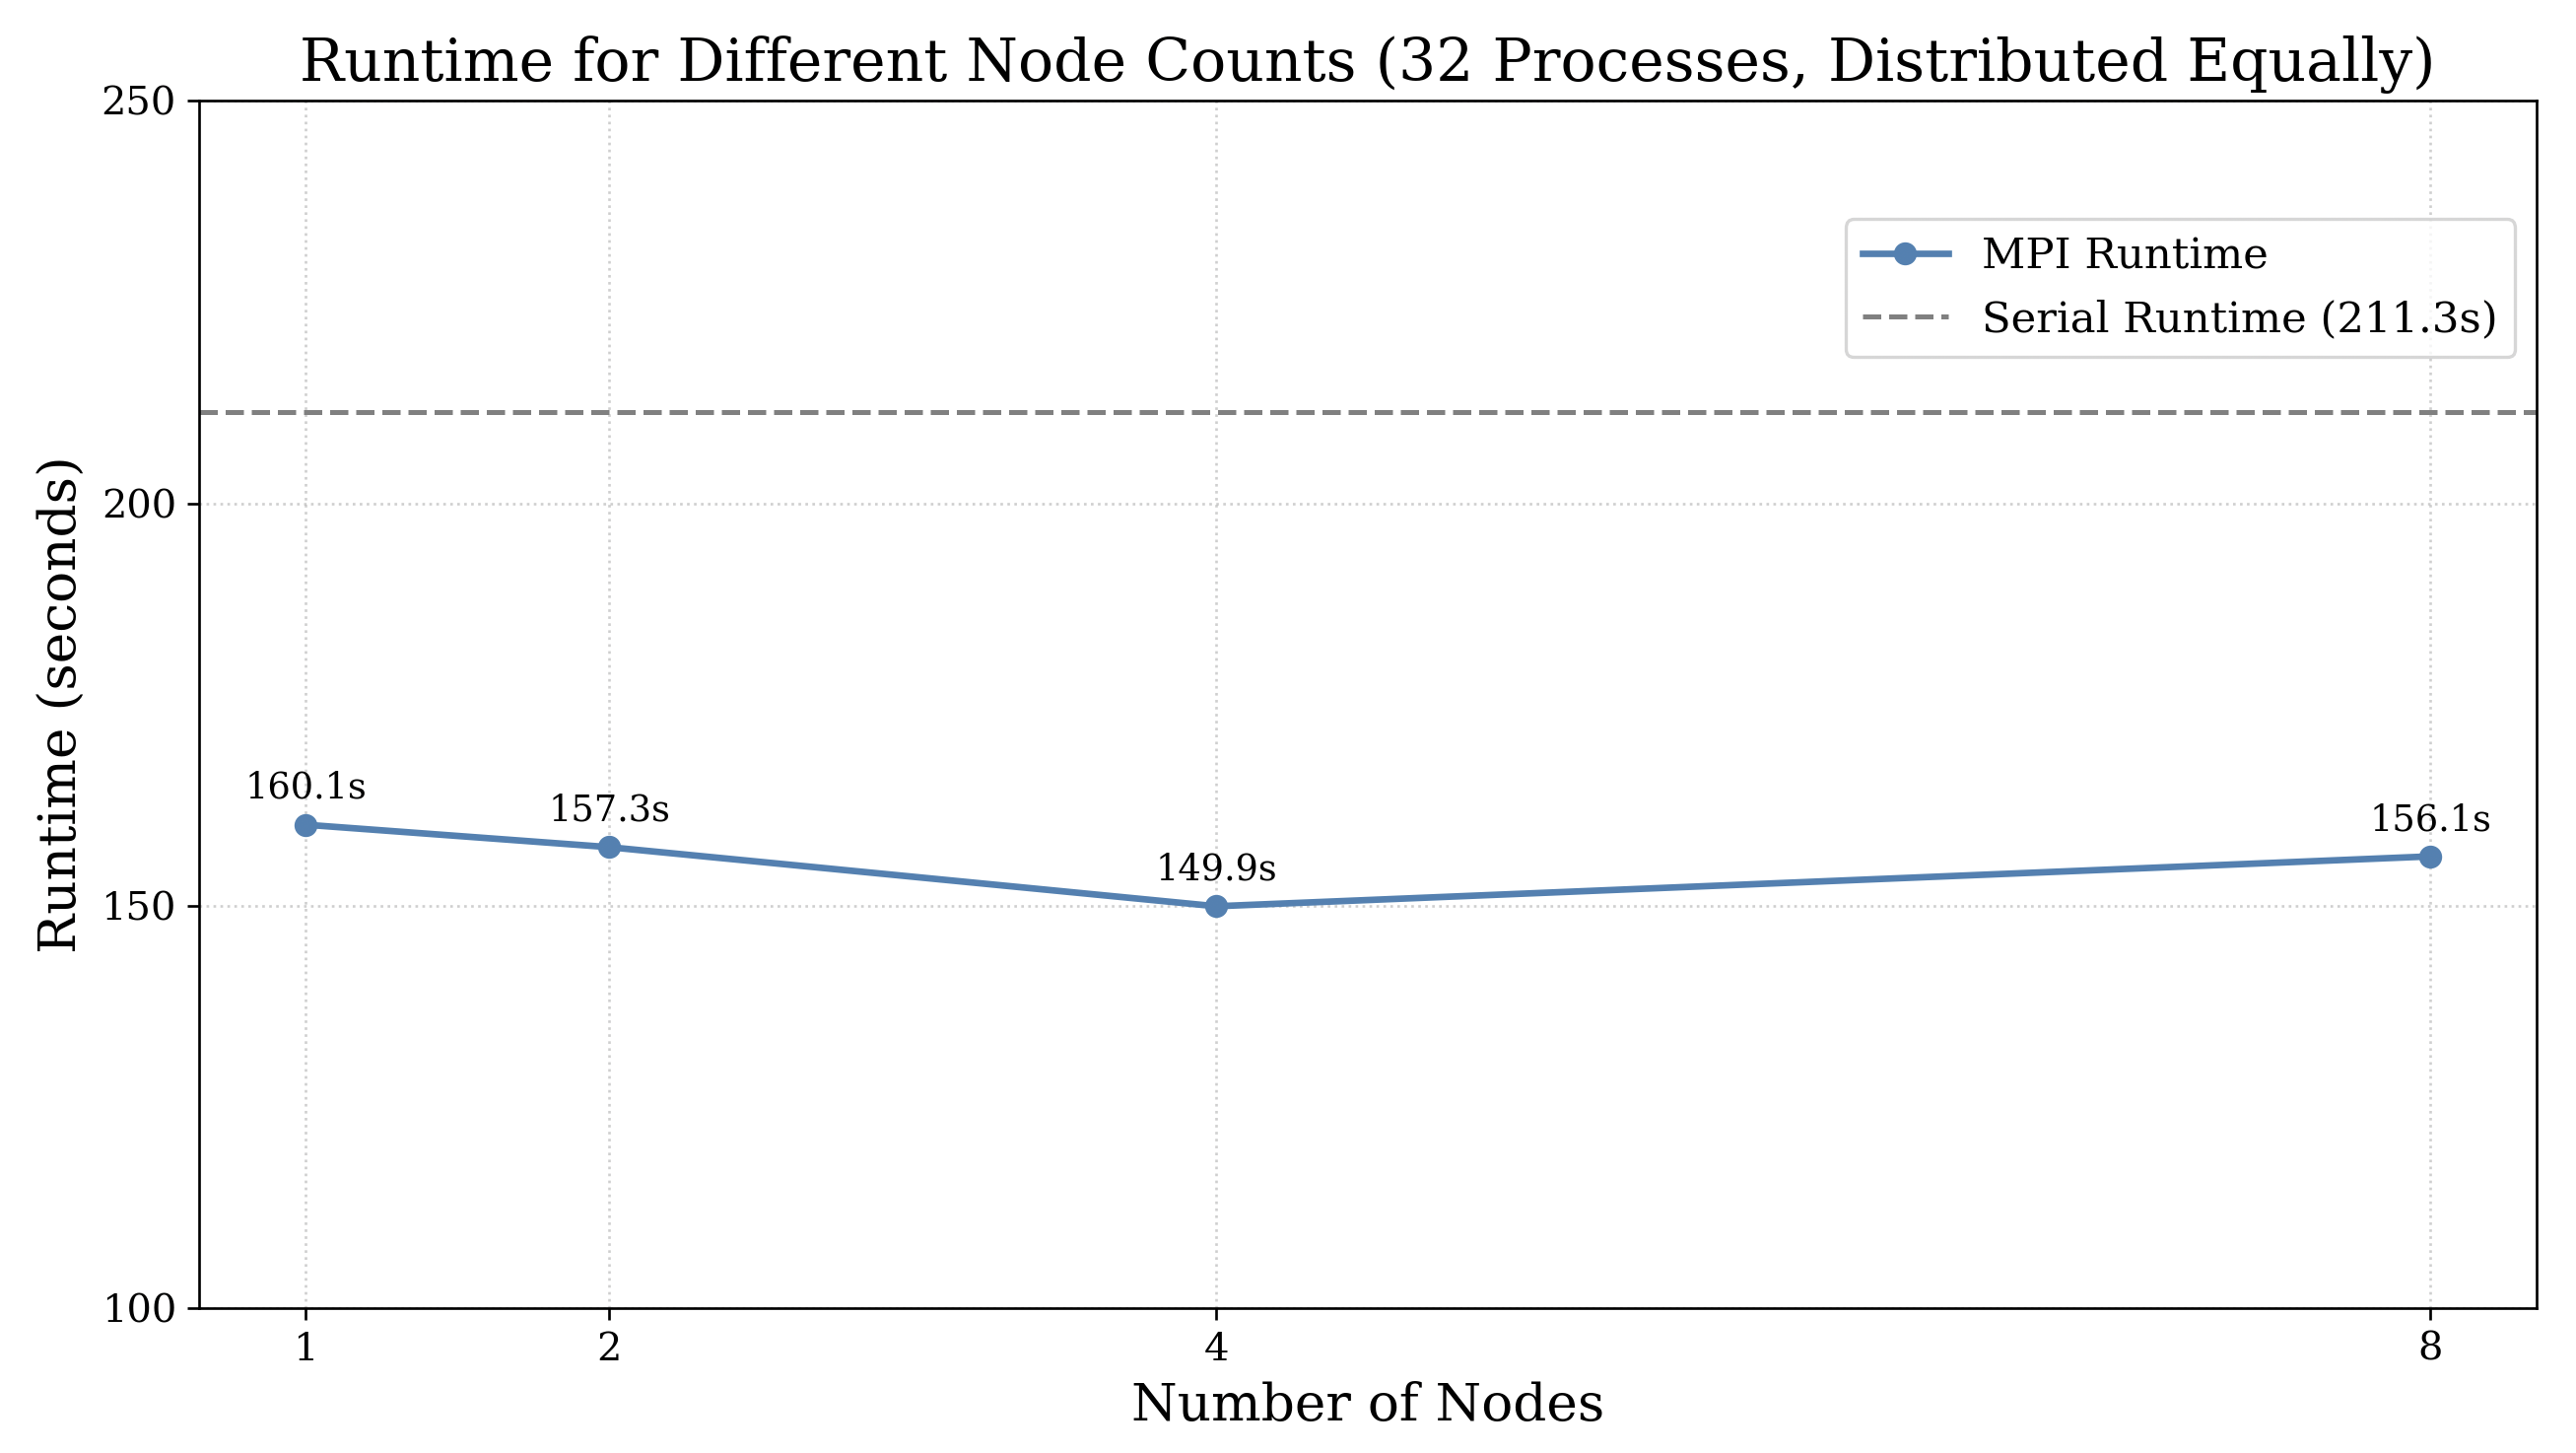
\includegraphics[width=0.9\textwidth]{img/ex1/diff_node_counts}
  \caption{Serial vs MPI Comparison for Different Node Counts}
  \label{fig:ex1_node_counts}
\end{figure}

As can be seen from the figure, the runtime across different node counts is considerably lower than the serial runtime on 1 node. This indicates that despite the possible network-overhead involved with communication over different nodes, the benefits of MPI parallelism compared to the serial version far outweigh the potential downsides. The runtime gradually decreases till 4 nodes, and then slightly increases at 8 nodes. This seems to be in-line with our expectations: distributing across 2 or 4 nodes might help in reducing the load on a single node while keeping inter-node network communication within a reasonable limit -- giving better runtimes. However, as the number of nodes increase to 8, so does the inter-network communication overhead, which slightly decreases the efficiency. 

However, we'd note that the trend doesn't seem to be as large as we had expected. To us, this might indicate that inter-network node communication might not be the leading factor contributing to the runtime of the MPI implementation. Replacing the blocking nature of \verb|Sendrecv| with \verb|Isend + Irecv|, which would allow us to overlap computation with communication, and other optimizations can further be applied to improve the runtime even more across several nodes. 

\subsubsection{Strong and Weak Scaling}
\begin{figure}[H]
  \centering
  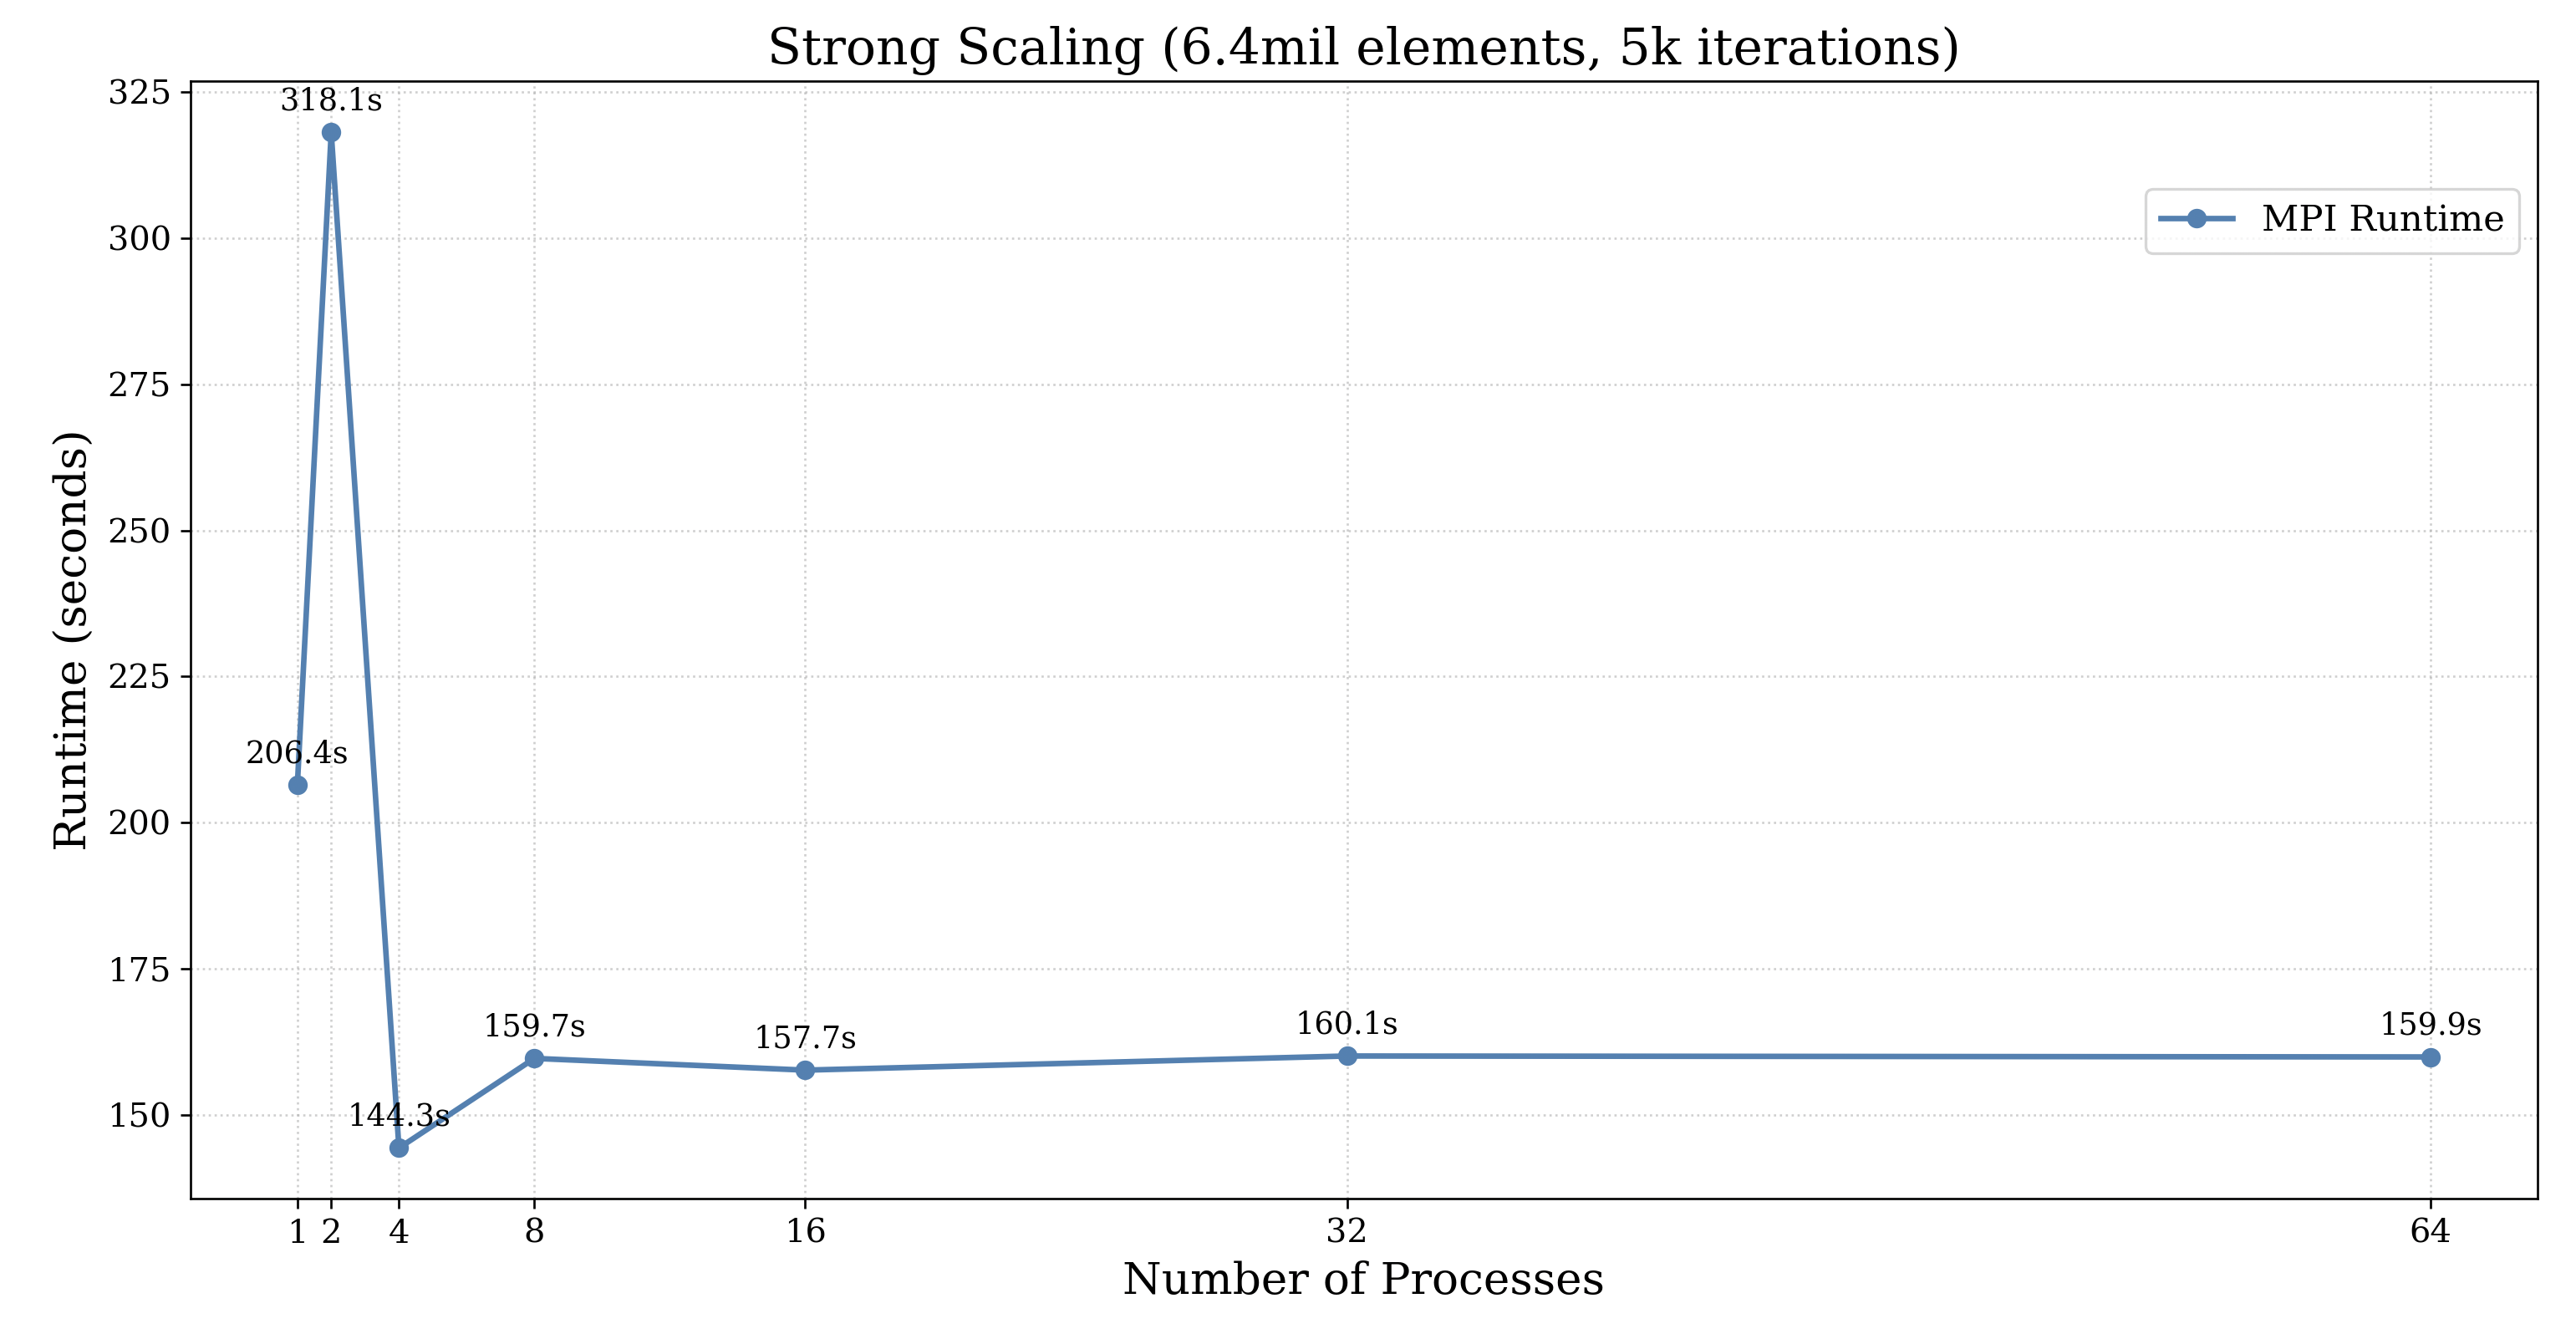
\includegraphics[width=0.9\textwidth]{img/ex1/strong_scaling}
  \caption{Strong Scaling}
  \label{fig:ex1_strong_scaling}
\end{figure}

The Strong-Scaling Test -- keeping the overall problem size constant while increasing the number of processes -- was already performed when varying the process counts. We present the graph again in Figure \ref{fig:ex1_strong_scaling} but refrain from repeating our analysis which can be found in Section \ref{sec:diff_process_counts}. 


The Weak-Scaling Test -- where the problem size per process is the same as the number of processes increase -- was performed by fixing 100k elements of the global array per process and 5k iterations. The job-script for this test was \verb|run_sim_weak_scaling.sh|. Figure \ref{fig:ex1_weak_scaling} presents the runtime output. 
\begin{figure}[H]
  \centering
  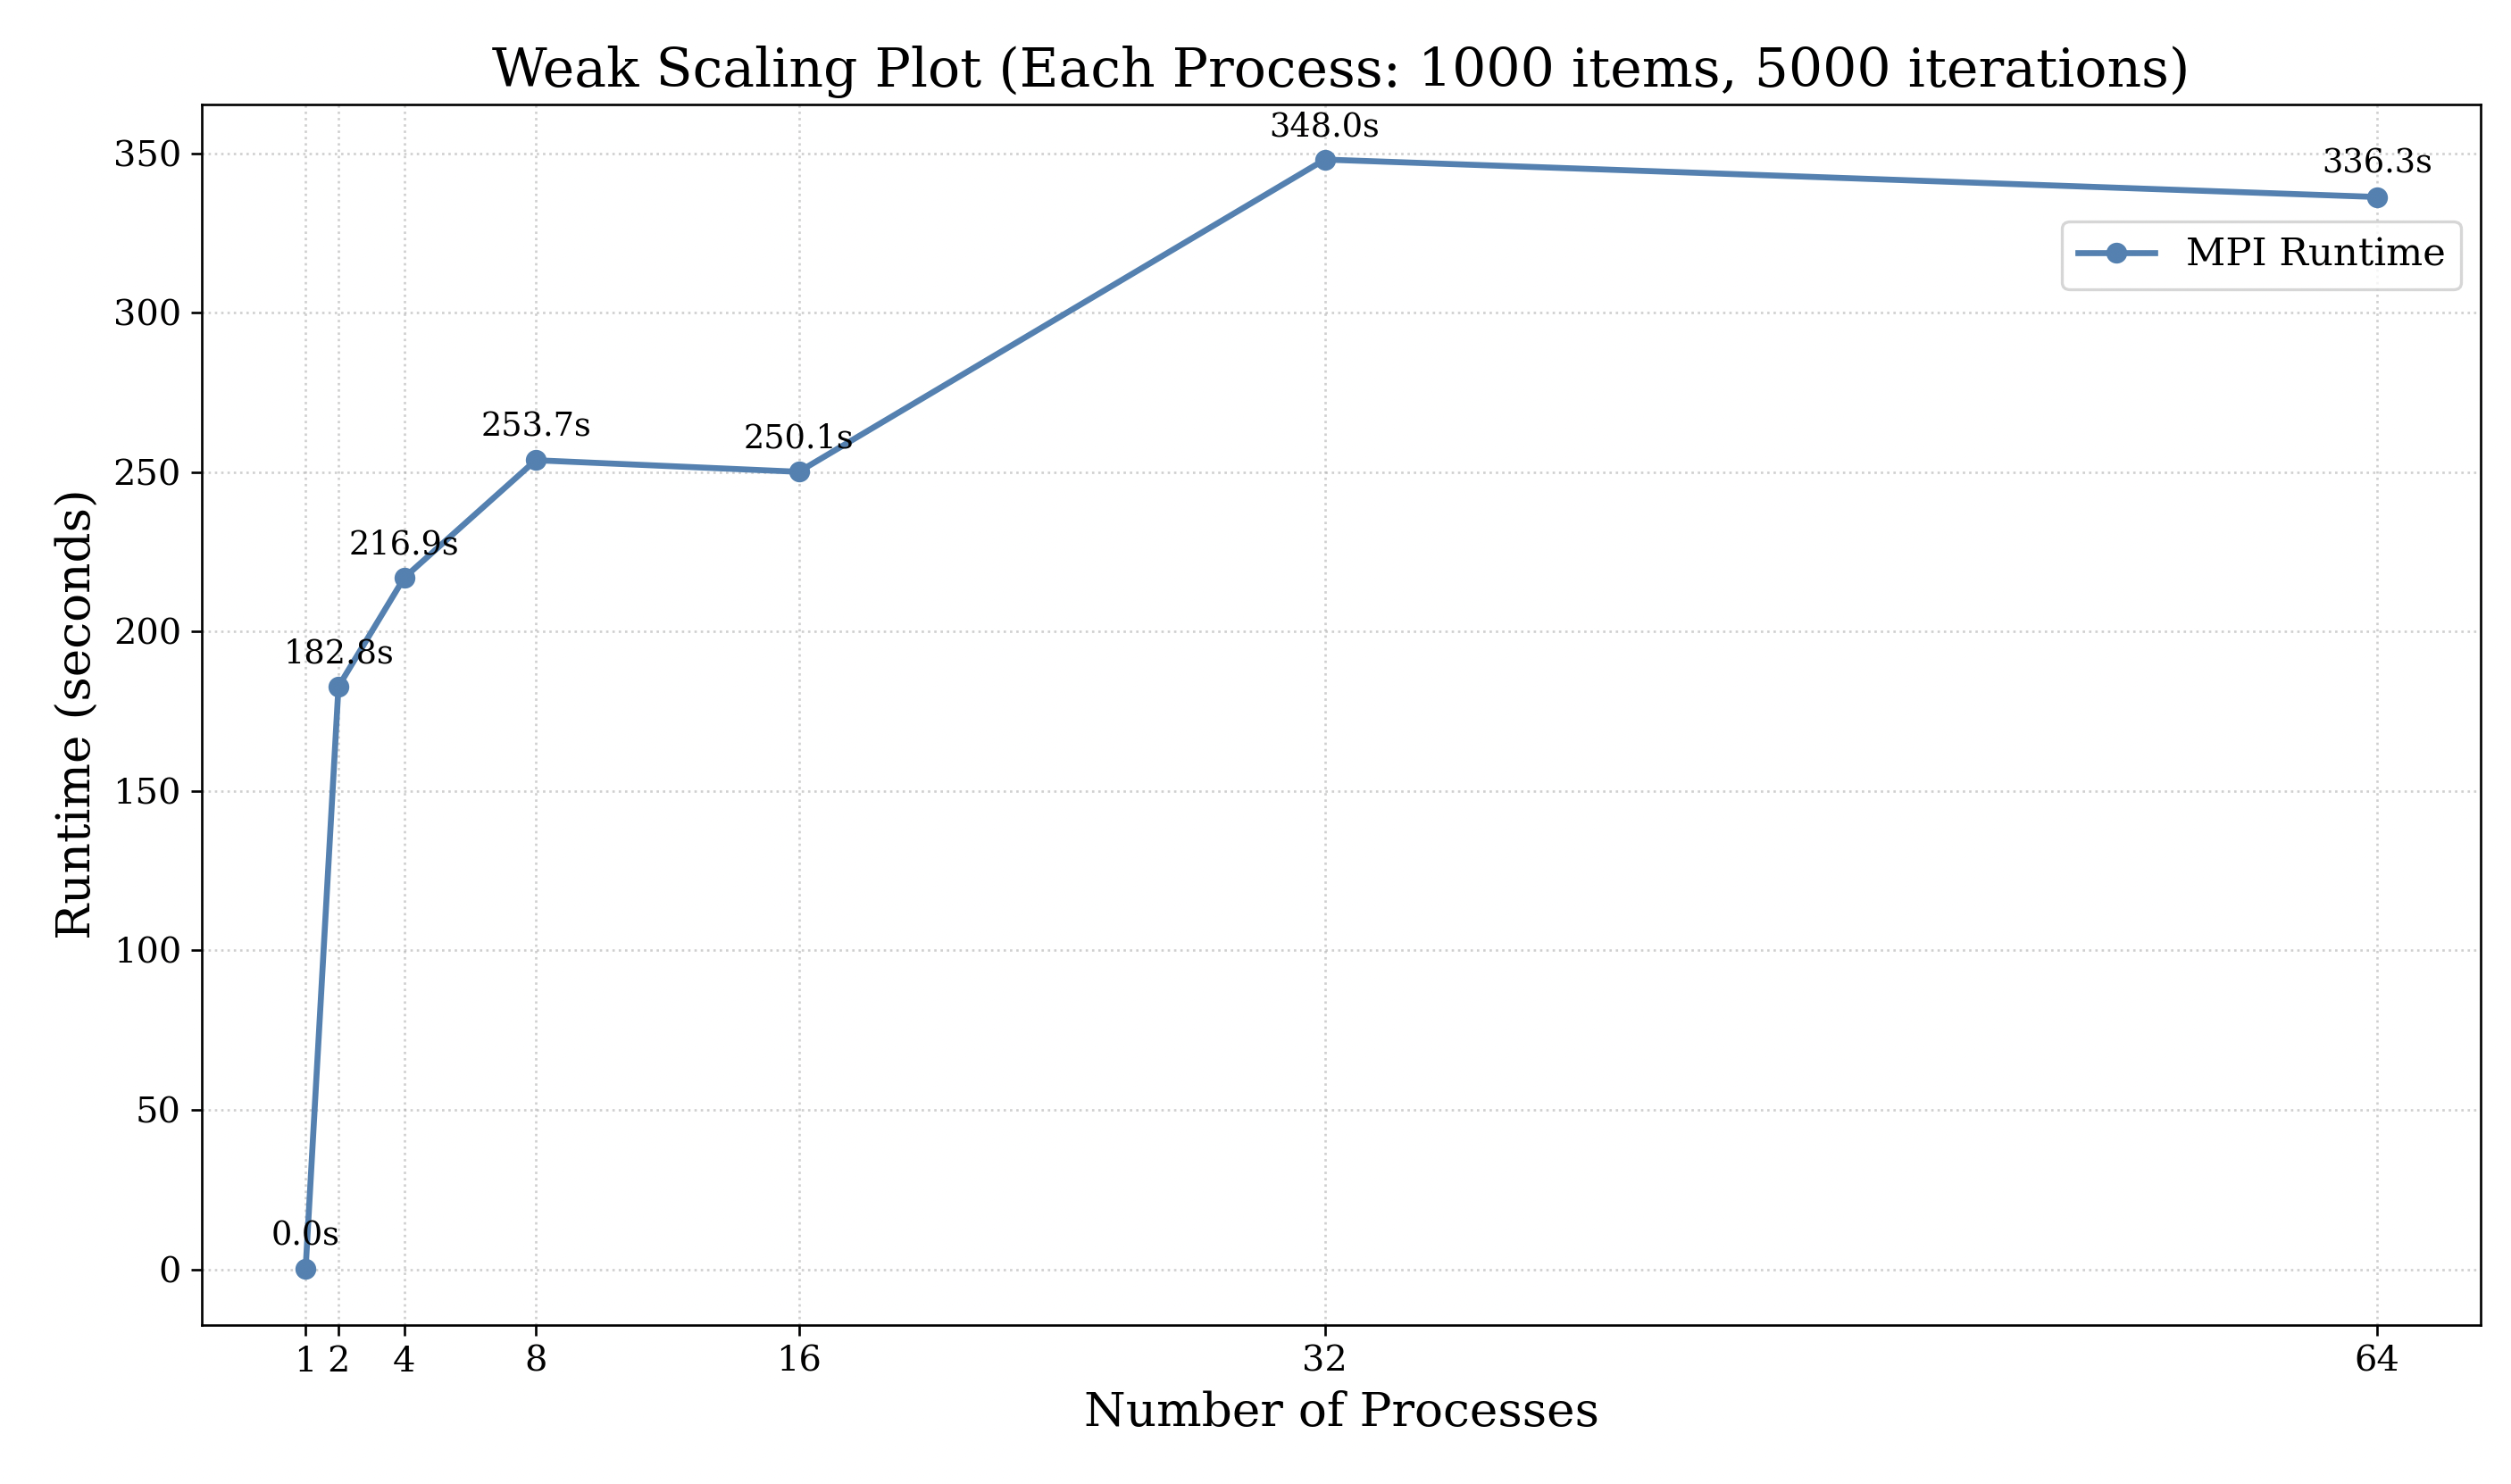
\includegraphics[width=0.9\textwidth]{img/ex1/weak_scaling}
  \caption{Weak Scaling}
  \label{fig:ex1_weak_scaling}
\end{figure}
The ideal scenario of a weak-scaling test to us would be similar runtimes as the number of processes (and thus the problem size) increases. This is because such a behaviour would indicate that larger problem sizes can be efficiently solved by increasing the number of resources (processes in our case) available to tackle them. Based on our understanding, the results we obtain largely adhere to the this ideal scenario.

We see a sharp increase in the runtime on going from 1 process to 2 processes. This is within our expectations: as there is now communication and syncronization overhead involved with multiple processes in the picture. There is a noticeable decrease in the runtime on going from 2 to 8 processes, which to us is an excellent obseration -- as this would indicate that the implementation is scaling well: larger problem sizes can be solved even more quickly with larger processes available. The runtime then begins to increase slightly, reaching the range of 150-160 seconds again as we go to 64 processes.

We did observe a considerable variation in the observations we made to obtain the average runtimes plotted for 4, 8, and 16 processes. However, in each of our runs, the runtime did not exceed the 16-160 second range. 

In all cases (except for the case with 1 sole process, the reasoning for which we gave above), the runtime remains similar as the problem size increases with the number of processes -- which was our expected ideal behaviour. At times, it seems to even perform better: decreasing with an increase in the number of processes and the problem size (like with 4 and 8 processes). 

\section{Parallel Row Sum Computation using MPI Collectives}
We started by running the code in the seqential version:
The generated image looks as follows:
\begin{figure}[H]
  \centering
  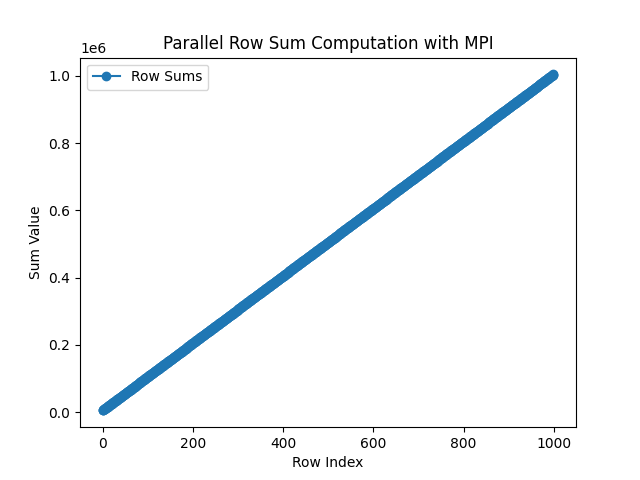
\includegraphics[width=0.9\textwidth]{img/ex2_seq}
  \caption{row summation using sequential implementation.}
  \label{fig:ex2_seq}
\end{figure}

To paralleise the code, we use \verb|MPI_Scatter(...)|.
To use MPI, we first initialise the application.

\lstinputlisting[language=C, firstline=62, lastline=66]{ex2/parallel_row_sum.c}

The main idea, is to distribute the matrix equally onto the available threads.
Our strategy is to split the matrix into chunks, each chunk contains an equal number of rows.
To achieve this, we first compute the chunk size, which is the number of rows each thread has to compute.
The basic formula for this is $\frac{N}{M}$, where $N$ is the number of rows and $M$ is the number of threads.
Because by default $N$ does not have to be divisible by $M$, we pad the matrix so that it has length $N^*$, where $N^* \mod M = 0$.
\lstinputlisting[language=C, firstline=75, lastline=77]{ex2/parallel_row_sum.c}
We initialize the matrix only on the root process and use scatter to distribute it to the rest of the threads.
This can be achieved by the following code:
\lstinputlisting[language=c, firstline=79, lastline=93]{ex2/parallel_row_sum.c}
Note, that the full matrix is only allocated on the root process!
The summation is then done on subsets of the matrix individually.
We gather all the solutions by using \verb|MPI_Gather(...)|:
\lstinputlisting[language=c, firstline=97, lastline=108]{ex2/parallel_row_sum.c}

The image looks identical to the sequential version:
\begin{figure}[H]
  \centering
  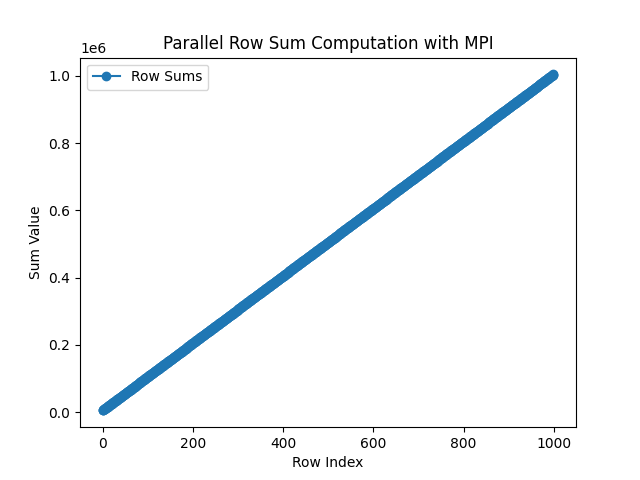
\includegraphics[width=0.9\textwidth]{img/ex2_para}
  \caption{row summation using parallel implementation.}
  \label{fig:ex2_seq}
\end{figure}

To compute the total sum, we first reduce the local result into a single local sum.
These we can then reduce globally using \verb|MPI_Reduce(...)|:
\lstinputlisting[language=c, firstline=110, lastline=113]{ex2/parallel_row_sum.c}
Note that for large matrices (depending on initialisation) this will lead to overflows!

We measured the performance in two different settings.
Figure \ref{fig:ex2_weak_scaling} depicts a so called weak scaling plot.
It describes the runtime of an increasing number of processors in regards to an increasing problem size, so that the work per processor stays consistent.

\begin{figure}[H]
  \centering
  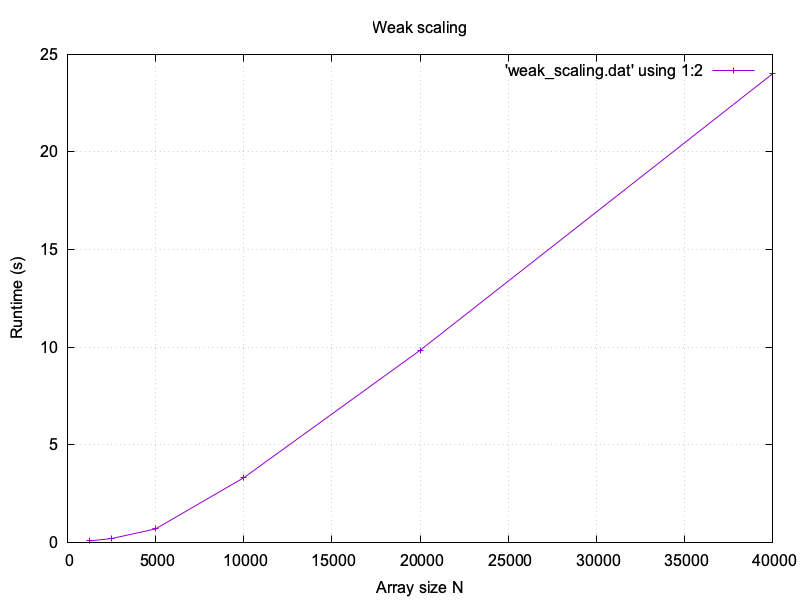
\includegraphics[width=0.9\textwidth]{img/ex2_weak_scaling}
  \caption{Weak scaling starting at 4 processors and N=1250}
  \label{fig:ex2_weak_scaling}
\end{figure}

We still see a strong increase in runtime.
As we discover in \ref{sec:ex3_ex2}, we see that the \verb|MPI_Scatter| overhead dominates the runtime if the problem.
For an increasing size of processors, this also means an increase runtime.

The scecond plot (\ref{fig:ex2_strong_scaling}) describes the string scaling. Here we keep the problem size fixed (Array of $10^8$ elements) distributed over $1..1024$ processors.
The most clear result, is that we cannot see any strong improvement for this problem size when scaling over 256 processors.
Also for small number of processors, the runtime first increases. This could be due to network congestion or the fact that introducing communication overhead outweighing the parallisation benefits.

\begin{figure}[H]
  \centering
  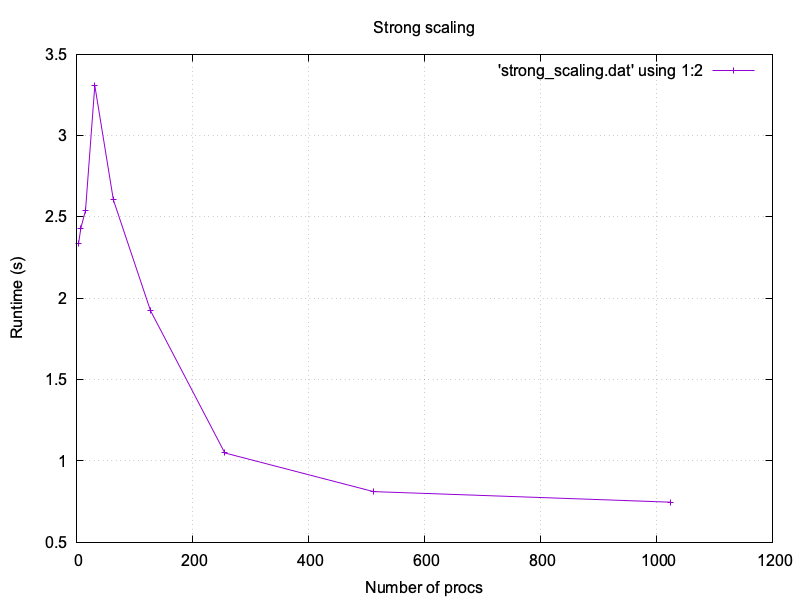
\includegraphics[width=0.9\textwidth]{img/ex2_strong_scaling}
  \caption{Strong scaling}
  \label{fig:ex2_strong_scaling}
\end{figure}

\section{Profiling MPI applications with Score-P and Vampir}

\subsection{Score-P with Exercise 1}
We used 4 Dardel Nodes with 8 processes per node, for a total of 32 processes. The array size (elements of \verb|u|) was 6.4million and the number of steps/iterations were 5k. We compiled the \verb|halo_parallel.c| file available \href{https://github.com/paulmyr/DD2356-MethodsHPC/blob/master/4_mpi/ex3/halo_parallel.c}{here} (with no writes to standard output or files) with the \verb|scorep| utility and ran the compiled file with the job script \verb|run_scorep_ex1.sh| available \href{https://github.com/paulmyr/DD2356-MethodsHPC/blob/master/4_mpi/ex3/run_scorep_ex1.sh}{here}. The results obtained can be found in the \verb|scorep-...| folder under the \verb|ex3/| directory of the repository. 

In Figure \ref{fig:ex3_ex1_scorep} we present the results of running the \verb|scorep-score| command on the \verb|.cubex| file in the \verb|scorep-...| directory. 

\begin{figure}[H]
  \centering
  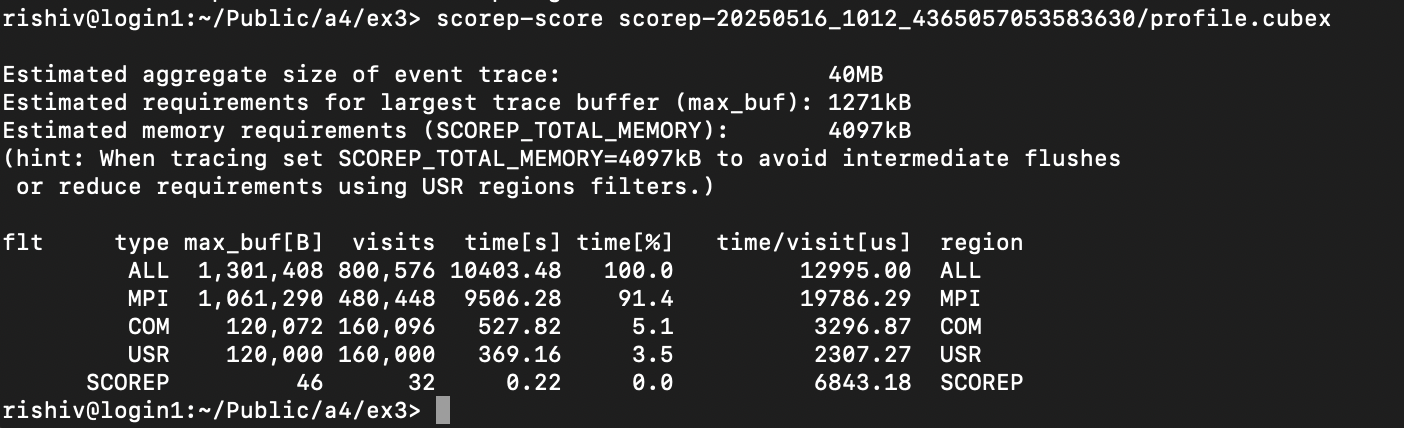
\includegraphics[width=0.9\textwidth]{img/ex3/ex1_scorep.png}
  \caption{ScoreP on Exercise 1 MPI Implementation}
  \label{fig:ex3_ex1_scorep}
\end{figure}

In total, there were around 480k MPI calls (the result of the \verb|visits| column), with a total of 9.5k seconds being spent in the MPI calls. There is some time spent in inter-network node communication as well (which we interpret as the result of the \verb|COM| row), but it is dwarfed by the large amount of time spent in MPI. We believe that this could be because of the blocking nature of \verb|Sendrecv| and could be improved by using non-blocking \verb|ISend| and \verb|IRecv| as a starting point, which would then allow us to perform even more optimizations (communication-computation overlap, among other things).

\subsection{Score-P with Exercise 2}
\label{sec:ex3_ex2}
\begin{figure}[H]
  \centering
  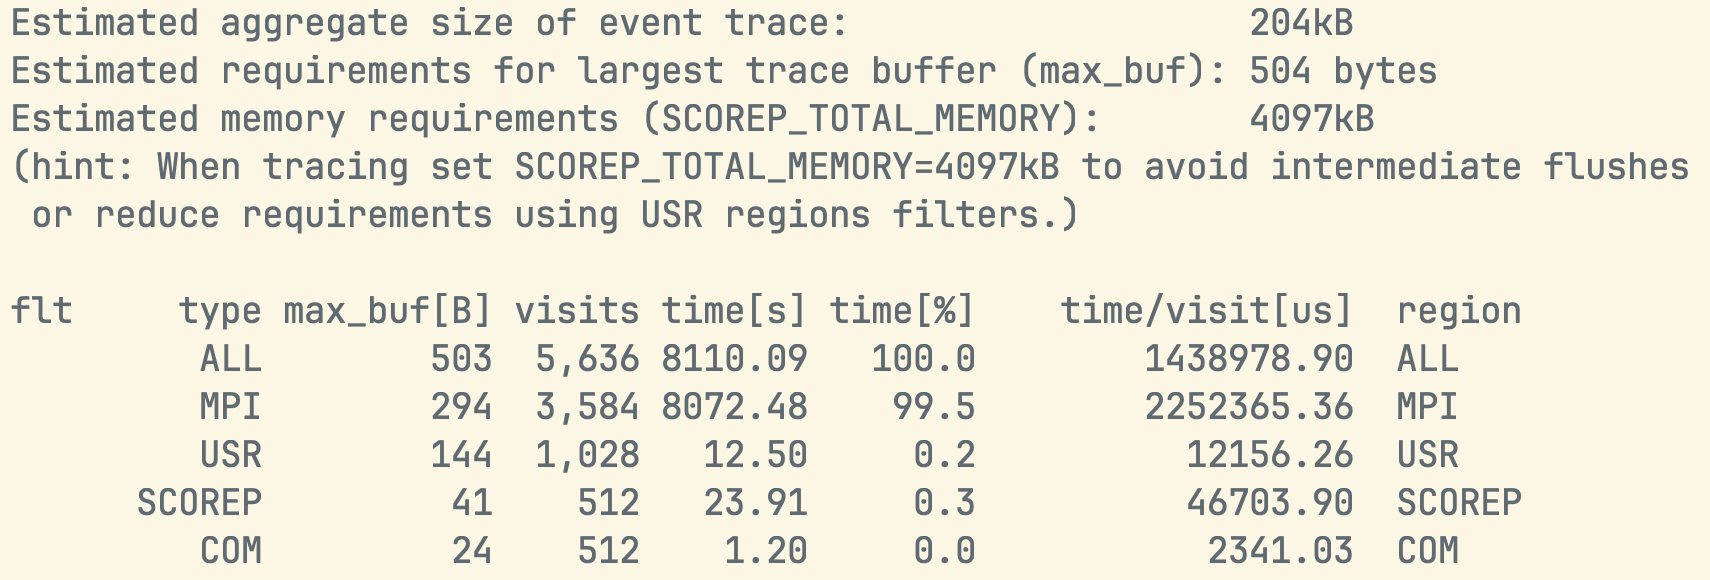
\includegraphics[width=0.9\textwidth]{img/ex3/ex2_scorep.png}
  \caption{ScoreP on Exercise 2 MPI Implementation}
  \label{fig:ex3_ex1_scorep}
\end{figure}

We can see that when running the code from exercise 2 on 4 nodes with 128 processors each, 99.5\% of the time is spent in MPI calls.
In total, 3,580 MPI calls were made which took over 8000s.
To us this indicates clearly, that the level of parallelism is too high.

\subsection{Vampir with Exercise 2}
\begin{figure}[H]
  \centering
  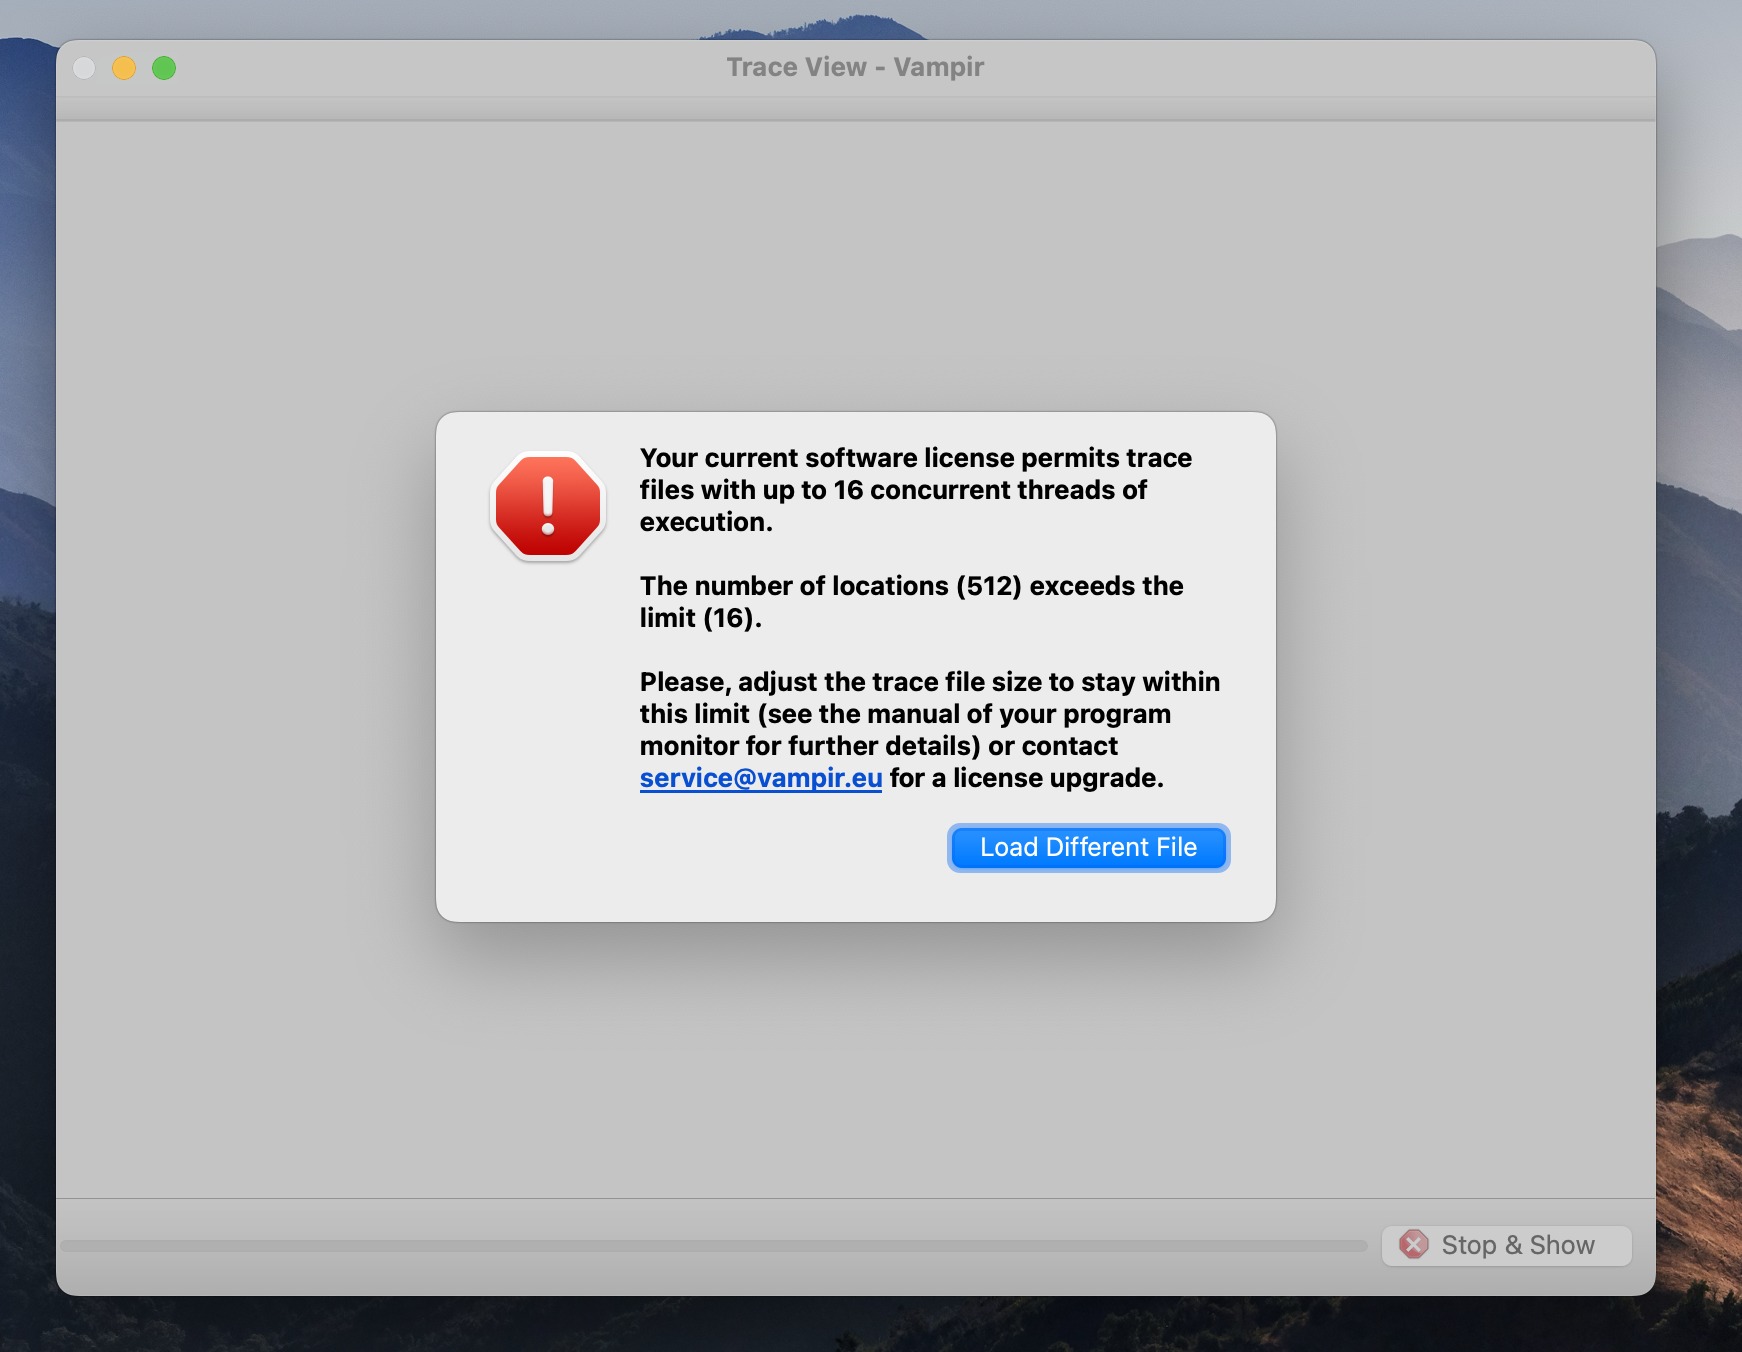
\includegraphics[width=0.9\textwidth]{img/ex3/ex3_license}
  \caption{Vampir License Issue}
  \label{fig:ex3_license}
\end{figure}

Due to the fact that Vampir only allows to process runs with up to 16 processes (see \ref{fig:ex3_license}), it is not possible for us to analyse the biggest run of Exercise two, which we performed up to 1024 processors...
However, when running the programm with 16 processors on a grid size of $40000^2$, we see can observe the following:

\verb|MPI_Scatter| is without question the biggest time sink of the computation. This indicates that the computation is heavily memory bound.
We can also see, that the initialisation consumes more time than the actual computation.

\begin{figure}[h]
  \centering
  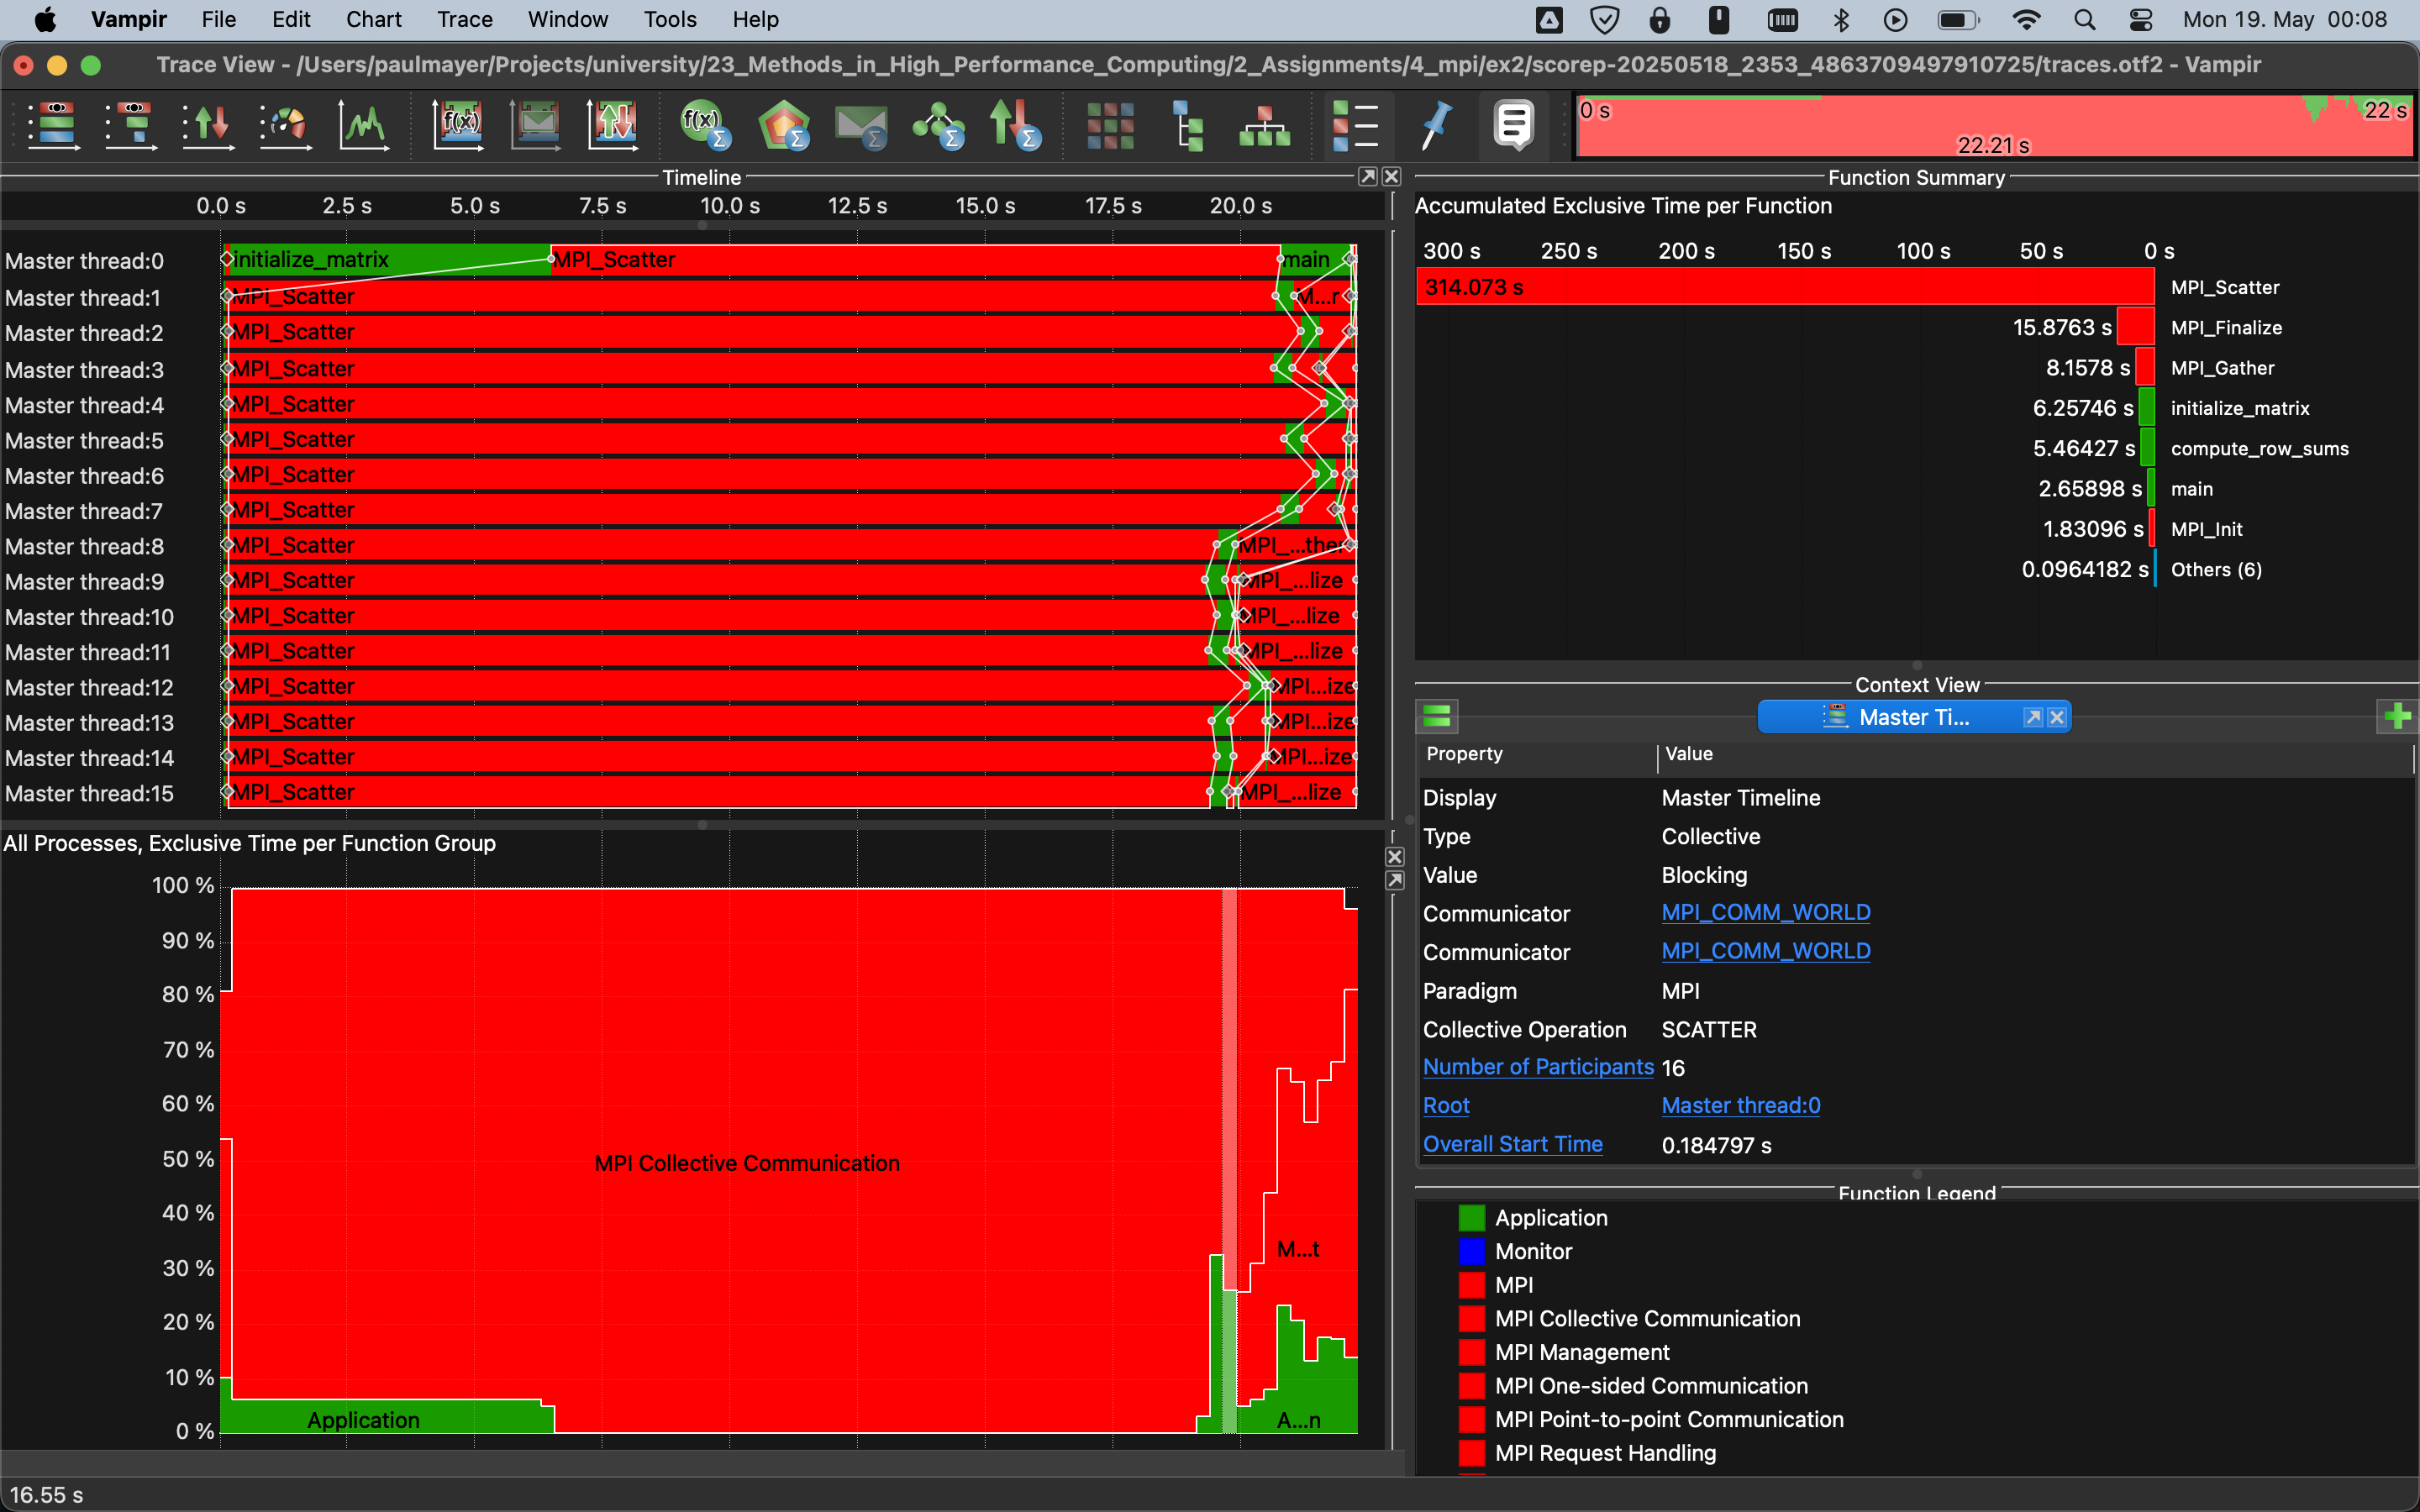
\includegraphics[width=0.9\textwidth]{img/ex3/ex3_vampir}
  \caption{Vampir profiling of row sum computation.}
  \label{fig:ex3_vampir}
\end{figure}

To lower the runtime of this program, the best approach would be perform the initialisation in a distributed fashion.
This significantly reduces the communication efforts, and also spreads the computational efforts on all the processors.

On the plus side, we don't detect any real load imbalances; however, this is mostly due to the fact that there is not a lot of load to begin with.
The computation at it's worst takes less than 5\% of the total runtime of any worker process.

\section{HPC Libraries -Matrix-Vector Multiplication using BLAS}
\subsection{Parallisation strategie and runtime}
The distribution strategy used in this exercise was similar as in exercise 2.
We sliced the array into equal sized chunks of consecutive rows, as well as distributed the vector to all processors.
Then each processor computed the Matrix-Vector Multiplication using BLAS, which was then gathered again on the main thread.
Because \verb|BLAS| is already highly optimised to run in parallel using shared memory, we actually saw a decrease in performance when distrbuting over the same node (instead of using the more cpus per task).
However, we were able to decrease the overall runtime by splitting the problem size over multiple nodes.

\begin{figure}[H]
  \centering
  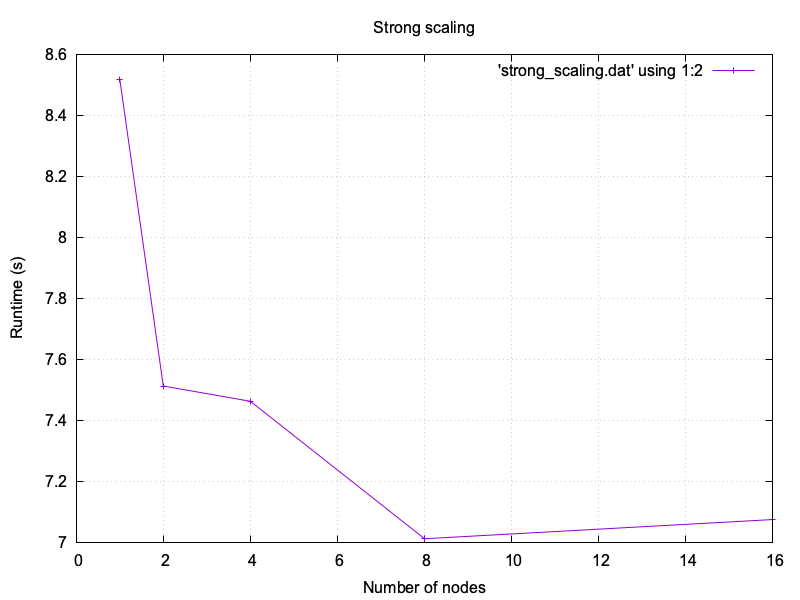
\includegraphics[width=0.9\textwidth]{img/ex4_strong_scaling}
  \caption{row summation using parallel implementation.}
  \label{fig:ex4_strong_scaling}
\end{figure}

Figure \ref{fig:ex4_strong_scaling} depicts the runtime over the number of nodes used.
It is a strong scaling plot, meaning the problem size remains identical at a matrix size of $40000^2$ elements.

\subsection{Verify correctness}
To verify correctness we visualise the output from the parallel run and the sequential run.
Figure \ref{fig:verification_graphs_ex4} shows that they are indeed the same.

\begin{figure}
     \centering
     \begin{subfigure}[b]{0.45\textwidth}
         \centering
         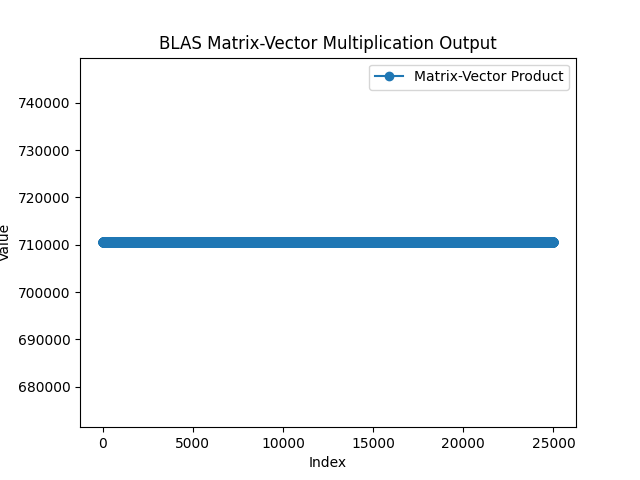
\includegraphics[width=\textwidth]{img/ex4_sequential}
         \caption{visualisation sequential result}
         \label{fig:ex4_strong_scaling}
     \end{subfigure}
     \hfill
     \begin{subfigure}[b]{0.45\textwidth}
         \centering
         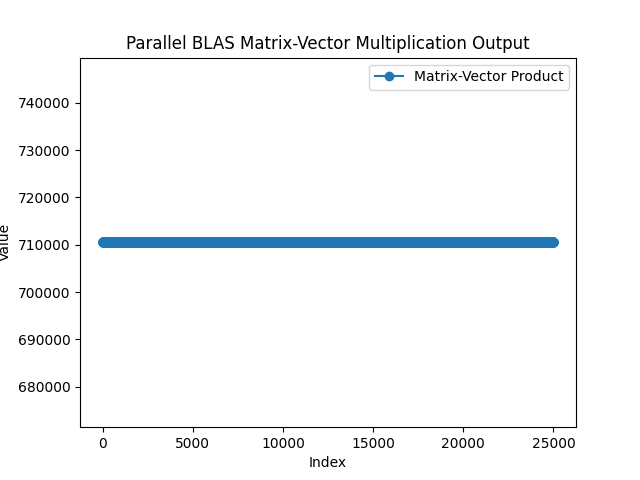
\includegraphics[width=\textwidth]{img/ex4_parallel}
         \caption{visualisation parallel result}
         \label{fig:ex4_parallel}
     \end{subfigure}
     \caption{Verification graphs}
     \label{fig:verification_graphs_ex4}
\end{figure}

\section{Bonus: 2D Game of Life with MPI and Non-Blocking Communication}
\subsection{MPI Implementation}
The MPI Implementation can be found in the \verb|life_parallel.c| file in the \verb|bonus/| directory for the project. Our implementation here follows the same ideas as the halo-exchange implementation of the wave simulation in Exercise 1. 

First, we delegate the process with rank 0 to initialize the grid in its entirety and then distribute it to the other processes. This is achieved by the \verb|initialize_and_send_grids| method \href{https://github.com/paulmyr/DD2356-MethodsHPC/blob/master/4_mpi/bonus/life_parallel.c#L34}{here}. Before doing this, however, we also create a 2D cartesian topology using \verb|MPI_Cart_create|, where the dimensions are obtained from calling \verb|MPI_Dims_create| beforehand. 

Following this, in each step of the main computation loop, we perform 2D halo exchanges of each cell with 8 of its neighbouring cells (since the grid wraps around). We create MPI data structures to efficiently exchange the rows and columns \underline{excluding} the 4 corners of the local grids. Additionally, the 4 corner exchanges are performed by exchanging individual values with the neighbouring ranks. For all these Halo exchanges, \verb|MPI_Irecv| and \verb|MPI_Isend| are used, as desired. We initiate all receive calls first, to ensure that the receiving process can immediately use the information as soon as it arrives. Additionally, the use of different flags for the different \textit{directions} in which the information was exchanged was needed to ensure correct delivery of ghost cells. All of this logic, along with more extensive comments explaining the implementation, can be found in the \verb|perform_halo_exchange| method \href{https://github.com/paulmyr/DD2356-MethodsHPC/blob/master/4_mpi/bonus/life_parallel.c#L119}{here}. We use \verb|Waitall| to wait for these 16 requests to finish before proceeding. After performing the halo exchange, the main computation loop performs the alive/dead calculation for each cell present in the local grid of the process before proceeding to the next step.

At every 10th timestep, we publish the current state of the grid to a text file. To ensure that all processes are at the same step of the computation whenever this state is published, we use \verb|MPI_Barrier|, followed by the printing of the grid. The process with rank 0 collects the local grids from each process and then is responsible for producing the output to the file. This logic can be seen in the \verb|print_grid| function \href{https://github.com/paulmyr/DD2356-MethodsHPC/blob/master/4_mpi/bonus/life_parallel.c#L192}{here}. Even if no output is written to file (which was done to get the runtimes), we have a \verb|MPI_Barrier| at the end of the main computation loop, followed by a \verb|IRecv| and \verb|ISend| calls at the root (rank 0) and other processes (respectively) to ensure that the final result is accumulated even if not printed.  

\subsection{Correctness of Parallel Implementation}
We used a grid size of $4096 \times 4096$ with 100 steps for the simulation.

Using the provided graphing file (\verb|visualize_grids.py|) to generate the visualizations and observed that for any given timestamp, the associated parallel and serial grid appears to be the same. We present 3 different visualizations: at timestep 0, 50, and 101 (after the loop simulation) in Figure \ref{fig:bonus_vis}. In addition to these visualizations, we automate the checking using the \verb|verify_outputs.sh| script. Like its counterpart in Exercise 1, running \verb|sh verify_outputs.sh| computes the diff between a timestep's parallel and serial outputs and ensures they have the same content.

\begin{figure}
\centering
\begin{subfigure}{0.4\textwidth}
    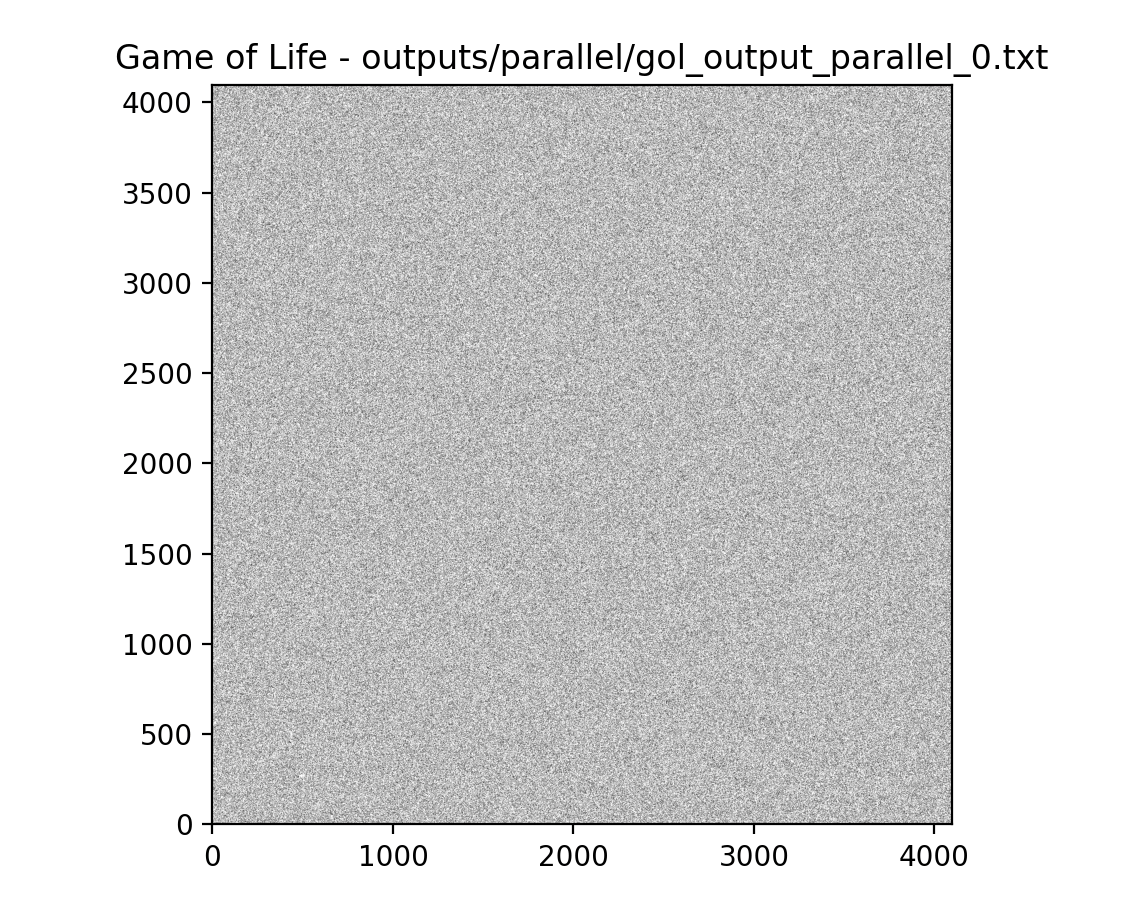
\includegraphics[width=\textwidth]{img/bonus/parallel_0.png}
    \caption{Parallel: Step 0}
\end{subfigure}
\hfill
\begin{subfigure}{0.4\textwidth}
    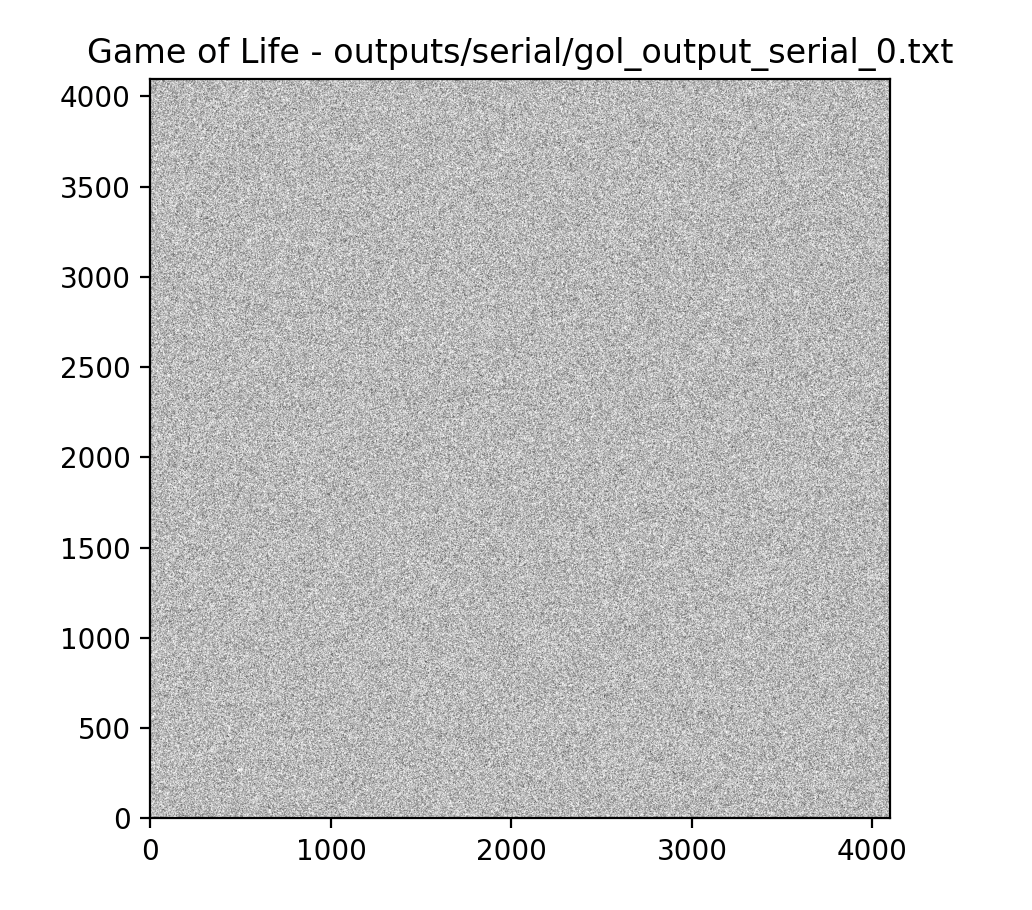
\includegraphics[width=\textwidth]{img/bonus/serial_0.png}
    \caption{Serial: Step 0}
\end{subfigure}
\hfill
\begin{subfigure}{0.4\textwidth}
    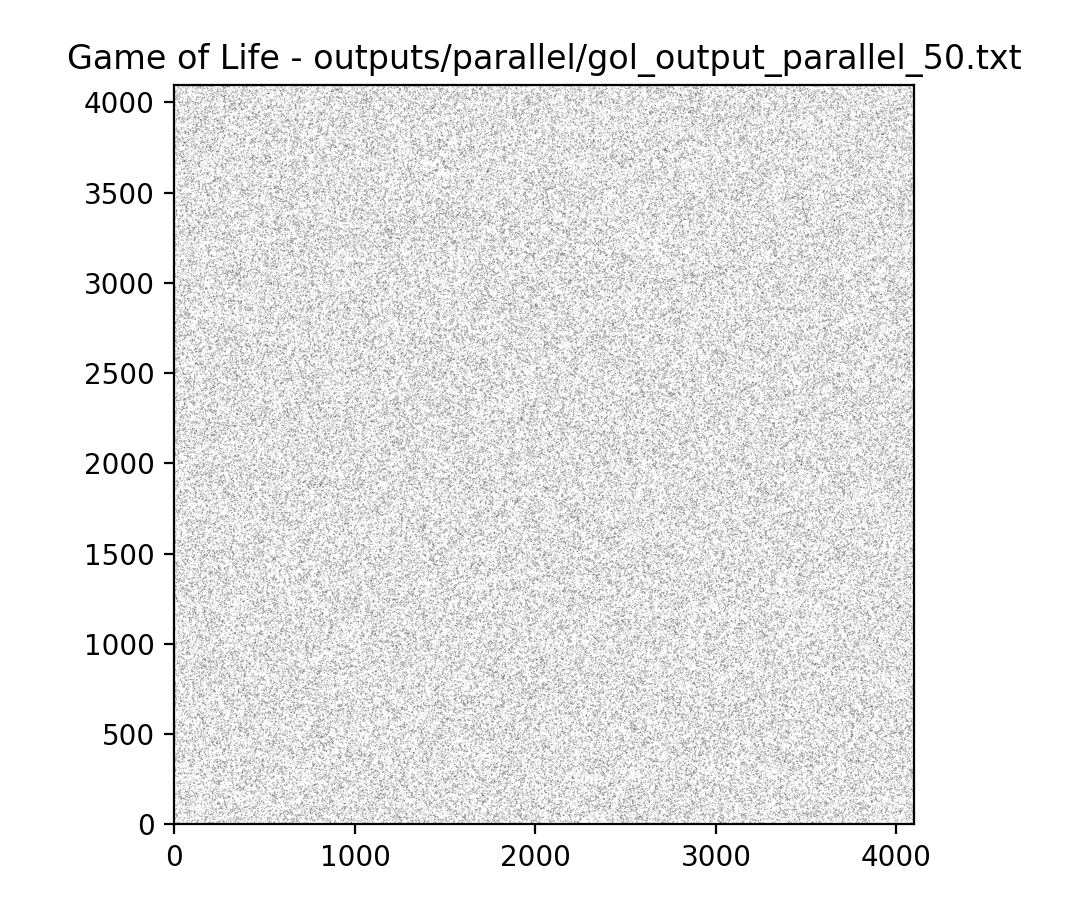
\includegraphics[width=\textwidth]{img/bonus/parallel_50.png}
    \caption{Parallel: Step 50}
\end{subfigure}
\hfill
\begin{subfigure}{0.4\textwidth}
    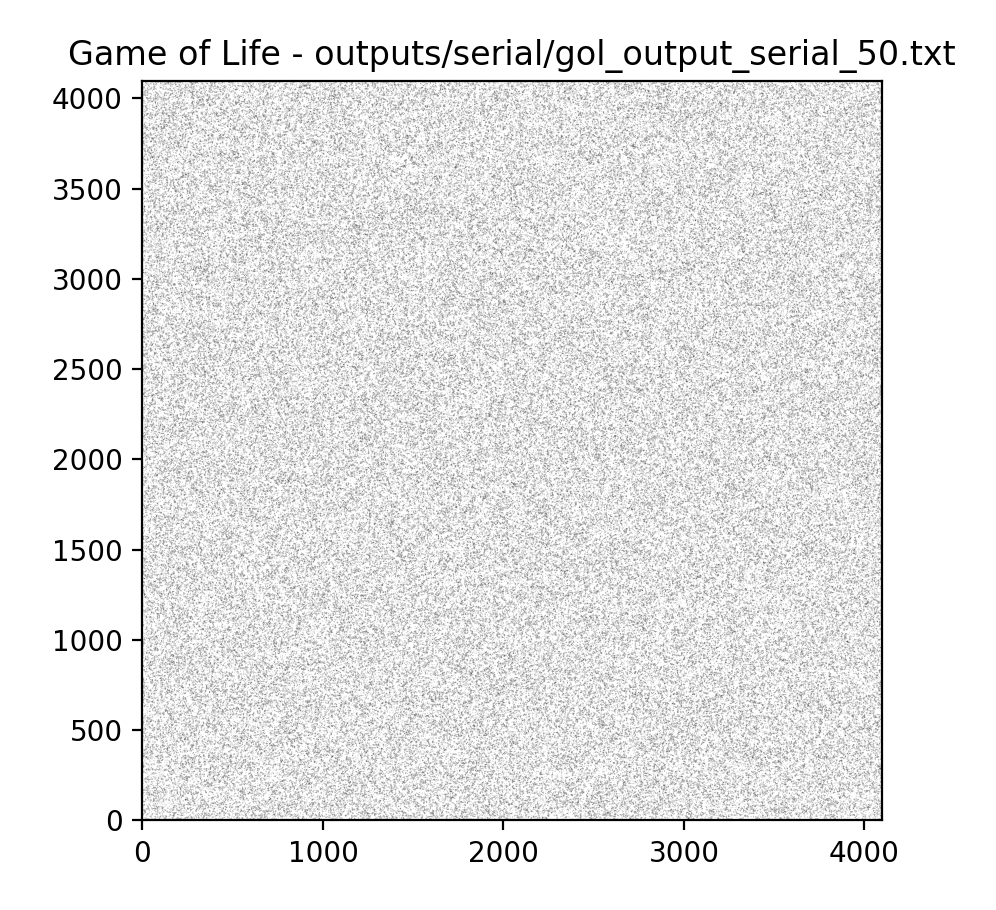
\includegraphics[width=\textwidth]{img/bonus/serial_50.png}
    \caption{Serial: Step 50}
\end{subfigure}
\hfill
\begin{subfigure}{0.4\textwidth}
    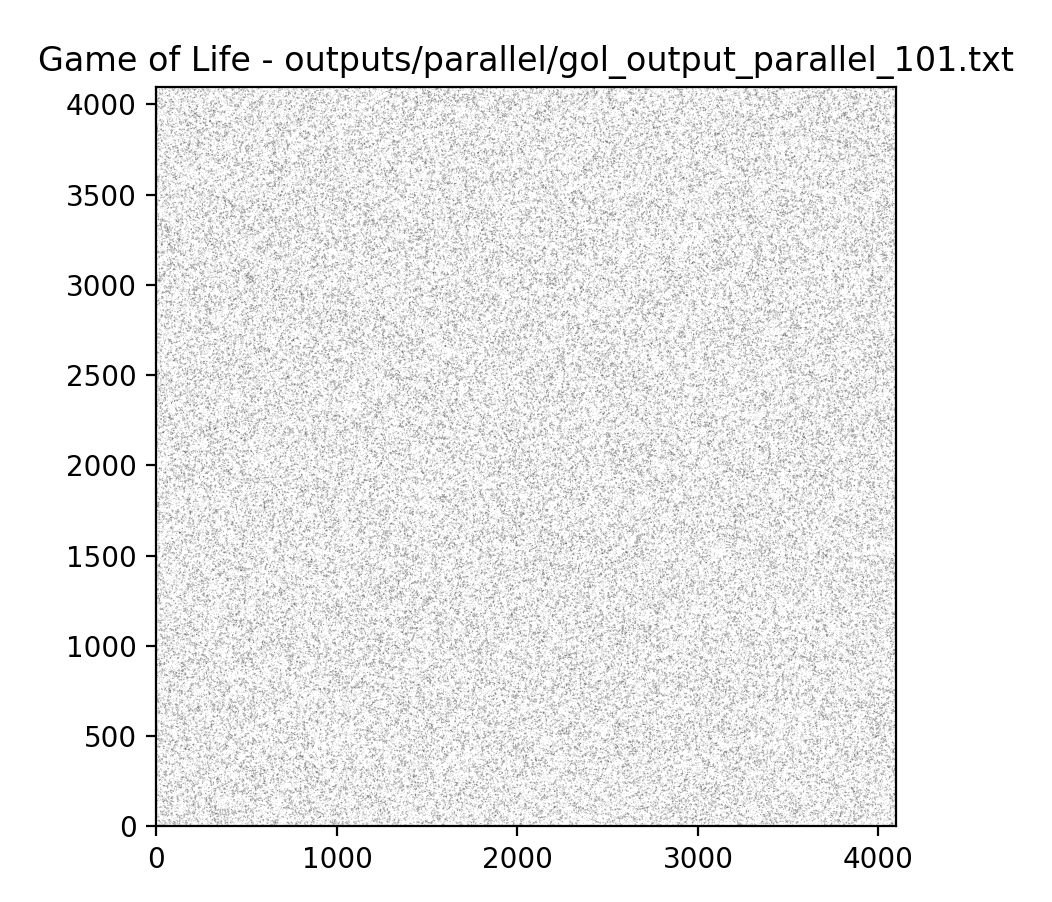
\includegraphics[width=\textwidth]{img/bonus/parallel_101.png}
    \caption{Parallel: Step 101}
\end{subfigure}
\hfill
\begin{subfigure}{0.4\textwidth}
    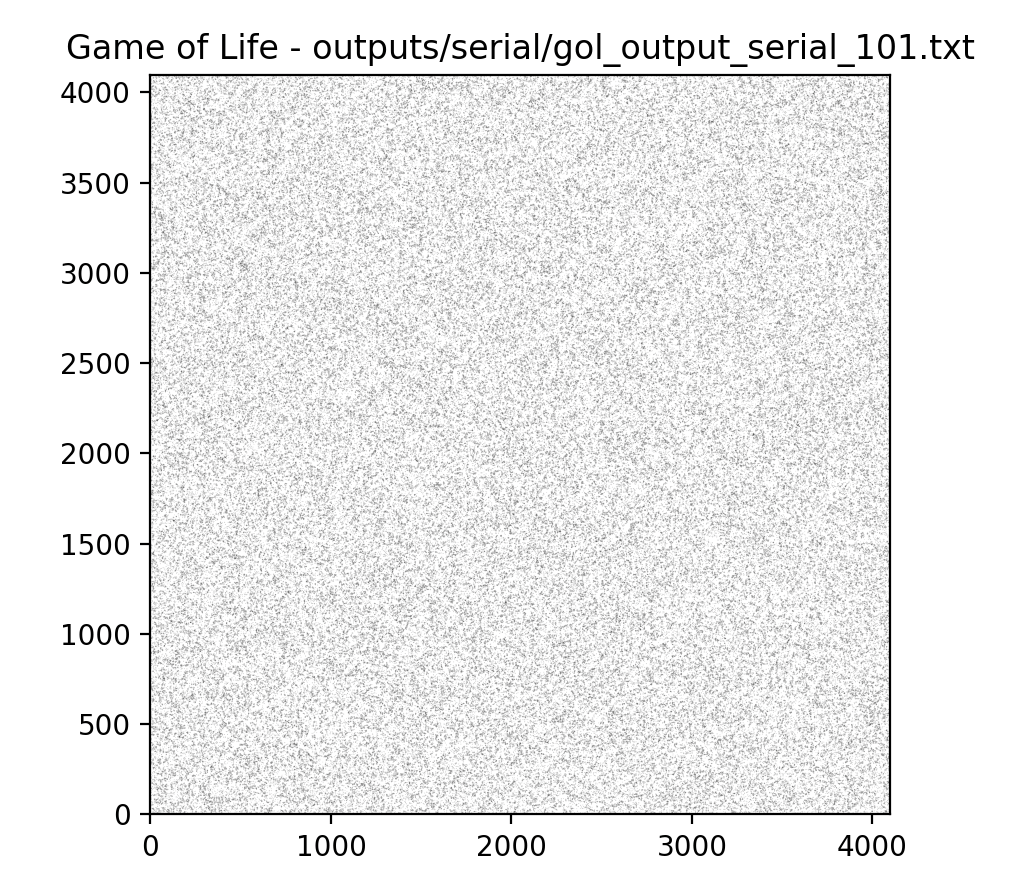
\includegraphics[width=\textwidth]{img/bonus/serial_101.png}
    \caption{Serial: Step 101}
\end{subfigure}
        
\caption{Screenshots at Different Timesteps for GoL Simulation}
\label{fig:bonus_vis}
\end{figure}

\subsection{Runtime Analysis}
We used a $4096 \times 4096$ grid and ran the simulation for 100 steps. With this setup, we tried different number of processes, all on a single node. Our full configuration for these runs can be found in the \verb|run_sim.sh| file present in the \verb|bonus/| directory of the repository. Note that we disabled all writes to files when measuring these runtimes, and we focus on timing the main computation loop. However, for the MPI implementation, we still have the \verb|MPI_Barrier| at the end of the loop followed by the collection of all local grids at the rank-0 process within the scope of the timing.

With this setup, the runtimes of the MPI implementation compared to the serial implementation can be seen in Figure \ref{fig:bonus_runtime}. The textual content from which the runtime was obtained can be found in the \verb|bonus/a4_bonus_output.txt| file of the repository.
\begin{figure}[H]
  \centering
  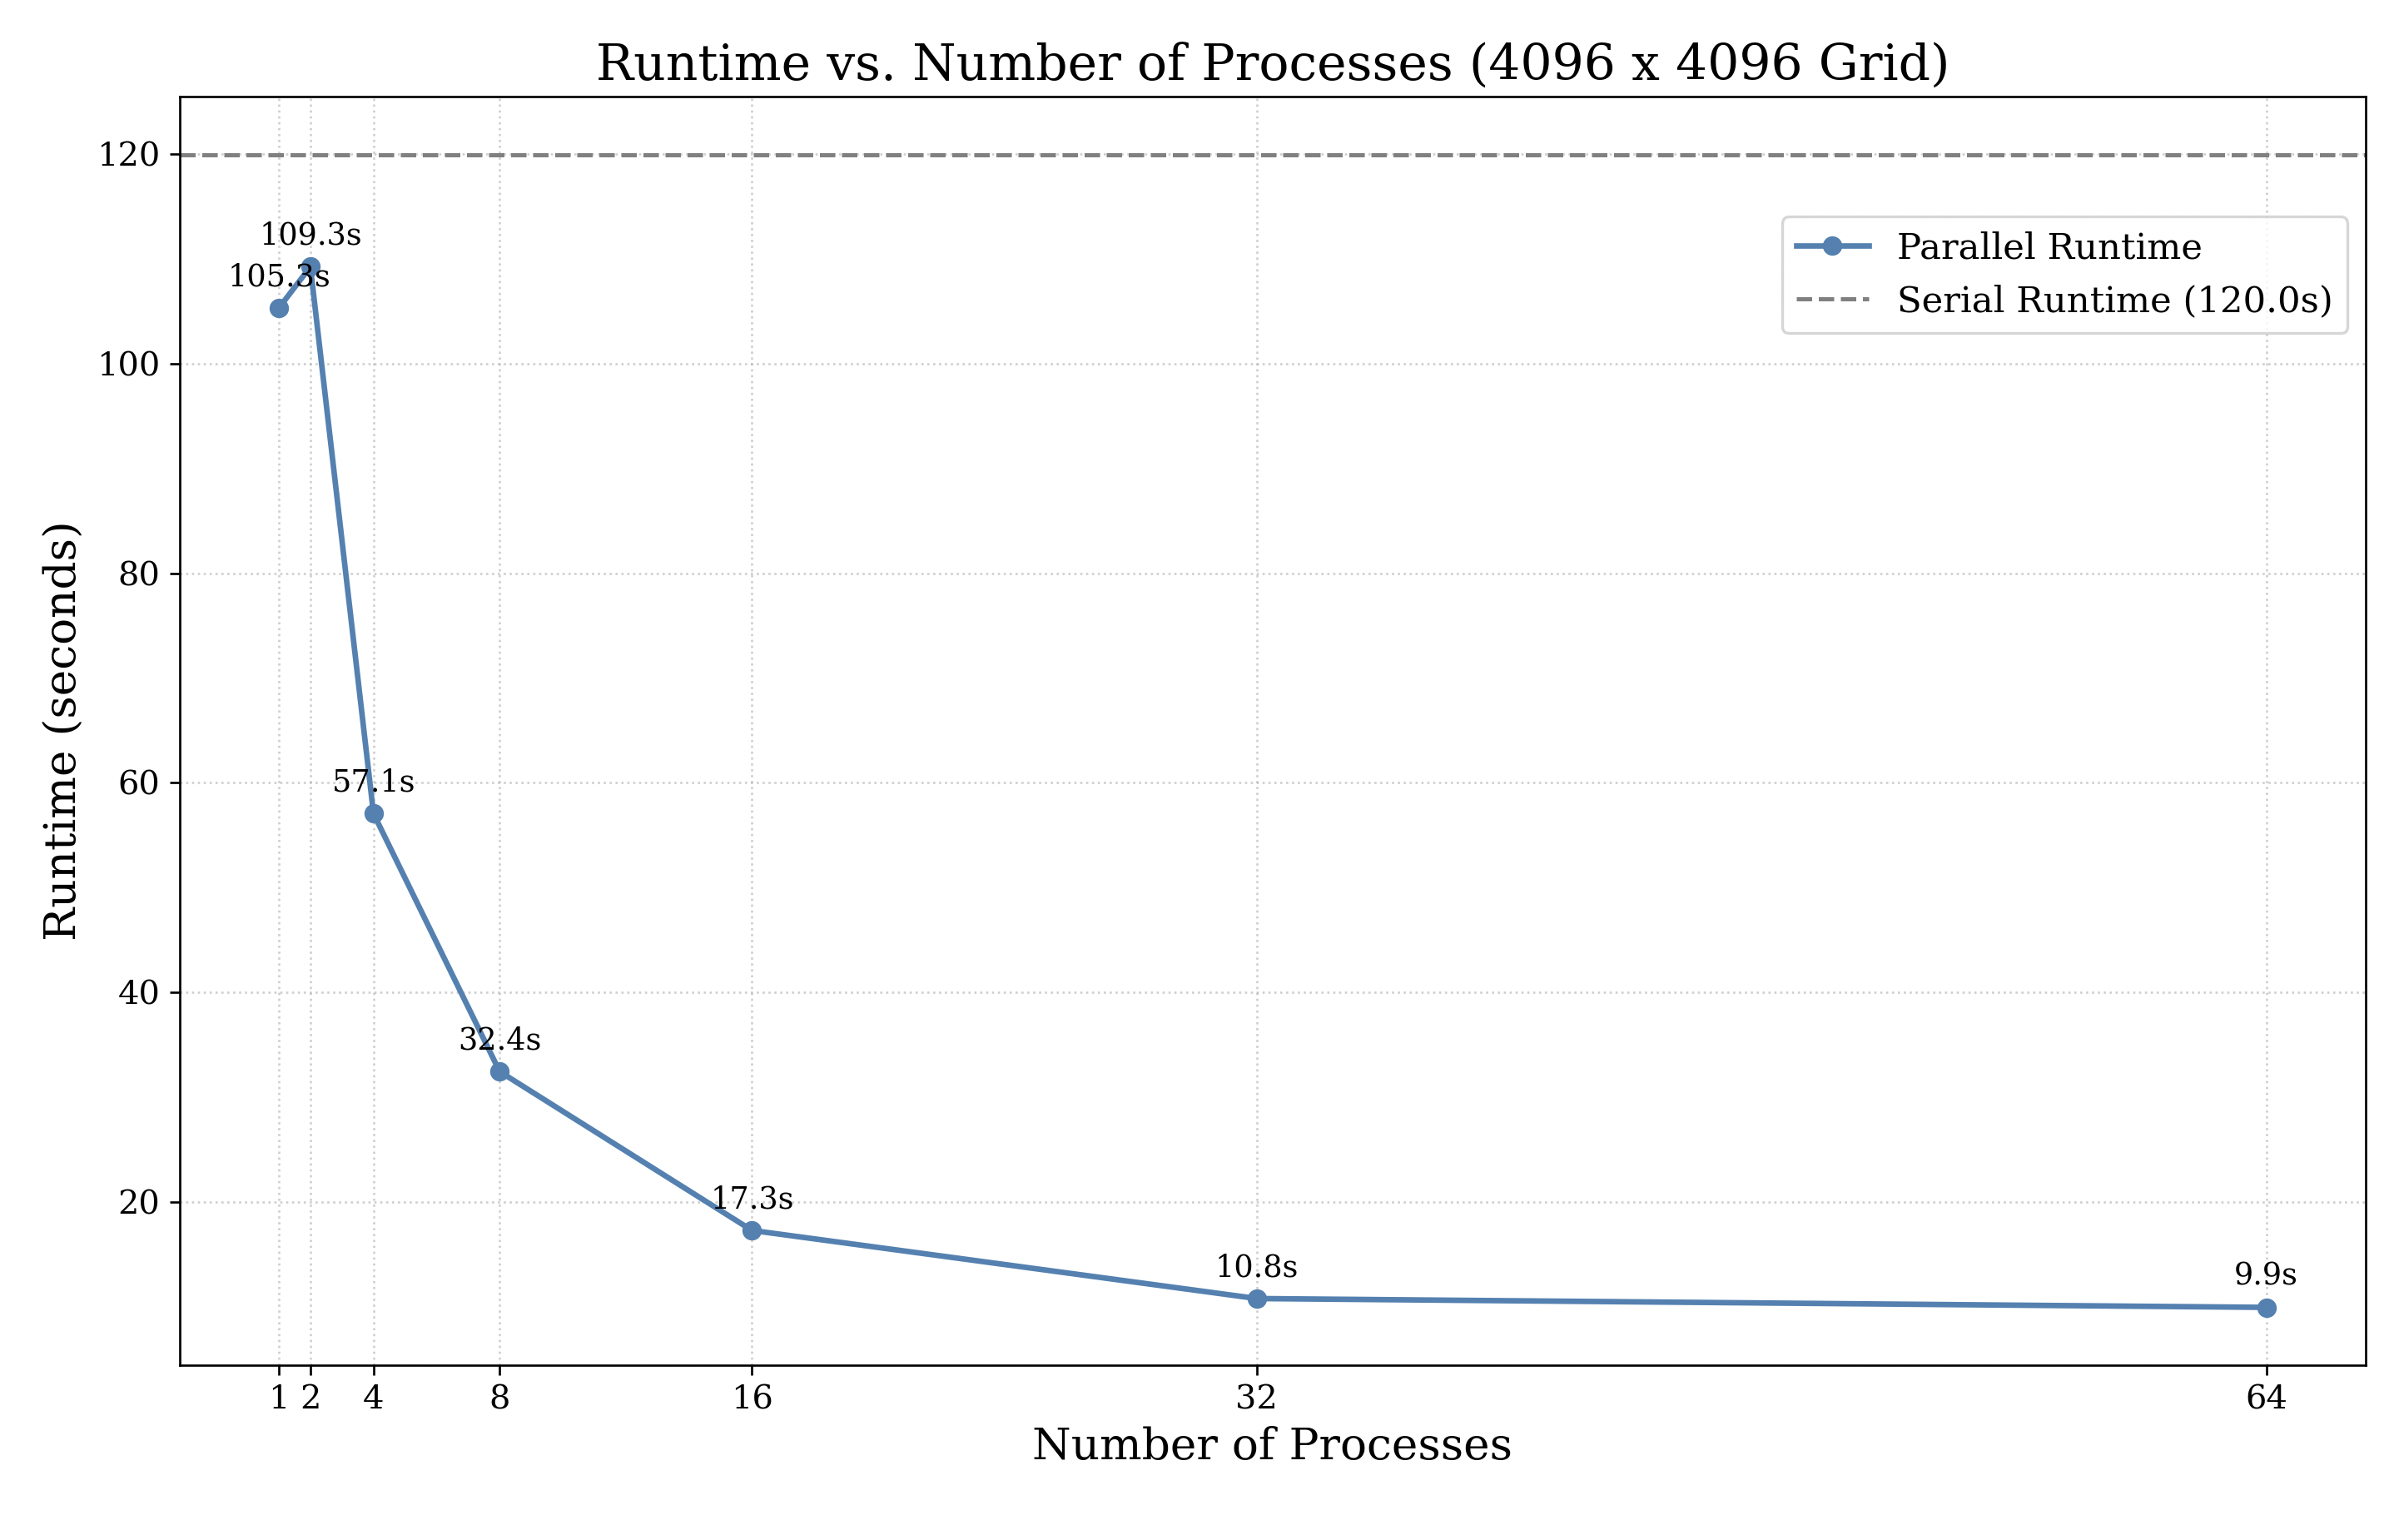
\includegraphics[width=0.9\textwidth]{img/bonus/runtime.png}
  \caption{GoL: MPI vs Serial Runtime Comparison}
  \label{fig:bonus_runtime}
\end{figure}

The runtime is greater for 1-2 processes compared to the serial implementation, likely because of the greater MPI overhead than the computational advantage offered by this low a number of parallel work. This is similar to the trend we saw in Exercise 1. However, as we increase the number of processes, we see a continual decrease in the runtime. The rate at which the decline in runtime happens decreases, however, there is a decline with an increase in the number of processes regardless. 

To us, this indicates that the implementation scales very well -- throwing a larger number of processes at the problem to parallelize the computation offers continual advantages (at least upto 64 processes). We believe that a reason for this could be the relatively large grid size (a 4096 square grid), meaning that the MPI overhead of ghost cell exchanges, barriers, and other related requirements is minimal compared to the advantages of working on large local grids in a parallel manner. One reason for this lower MPI overhead (compared to Excersie 1 for example) could be the use of non-blocking Send-Recv variations. With this, the processes are free to receive ghost cells from multiple processes instead of in a seemingly sequential manner. 

For future improvements, we believe we can improve this runtime even further by overlapping computation with communication. At the moment, we have a \verb|Waitall| call at the end of the halo-exchange routine. However, the ghost cells are not needed to compute the \textit{inner local setncils}, only the ones at the border. Thus, we could initiate the \verb|Irecv| and \verb|ISend| at a process, compute the inner stencil, then initiate a \verb|Waitall| for the 16 halo-exchange communications to finish, and then compute the borders before moving to the next iteration. This might lead to even better runtimes for the parallel implementation. We were very satisfied with the current state however and thus did not investigate the matter further at the moment, as even without the communication-computation overlap, the MPI implementation is very superior to the serial one. 


% content end
%###############################################################################

% \printbibliography

\end{document}
